% !TeX document-id = {c6282027-a510-40f1-b05e-2f558a6cd3f1}
% !TeX program = xelatex
% !TeX TXS-program:compile = txs:///xelatex/[--shell-escape]
%%%%%%%%%%%%%%%%%%%%%%%%%%%%%%%%%%%%%%%%%%%%%%%%%%%%%%%%%%%%%%%%%%%%%%%%
% TFM
% Universidad Politecnica de Madrid (ETSIAE)/ISAE Supaero
% Author: Sara Barrrasa Ramos
% Template by: José Manuel Requena Plens & Pablo José Rocamora Zamora
%%%%%%%%%%%%%%%%%%%%%%%%%%%%%%%%%%%%%%%%%%%%%%%%%%%%%%%%%%%%%%%%%%%%%%%%

%%%%%%%%%%%%%%%%%%%%%%%%
% FORMATO DEL DOCUMENTO
%%%%%%%%%%%%%%%%%%%%%%%%
% scrbook es la clase de documento
% Si se desea que no haya página en blanco entre capítulos añadir "openany" en los parámetros de la clase. Sino siempre los capítulos empezarán en página impar.
\documentclass[a4paper,12pt,titlepage]{scrbook}
\KOMAoption{toc}{bib,chapterentryfill} % Opciones del índice
\usepackage{scrhack} % Previene algunos errores
% Paquete de formato para scrbook. Con marcas, linea-separador superior e inferior
\usepackage[automark,headsepline,footsepline]{scrlayer-scrpage}
\clearpairofpagestyles		% Borra los estilos por defecto
%%
% Formato y contenido de la información de cabecera y pie de página
%%
% Información de capítulo en cabecera e interno
\ihead{{\color{gray30}\scshape\small\headmark}}	
% Número de página en cabecera y externo
\ohead{\normalfont\pagemark} 
% Número de página en pie de página y externo. Sólo en páginas sin cabecera
%\ofoot[\normalfont\pagemark]{}
%% 		
% Edición del contenido de las distintas partes de la cabecera
%%
\renewcommand{\chaptermark}[1]{\markboth{#1}{}} % Capítulo (Solo texto)
\renewcommand{\sectionmark}[1]{\markright{\thesection. #1}} % Sección (Número y texto)
\setkomafont{pagenumber}{} % Número de página (Sin nada añadido)

% Añade al índice y numera hasta la profundidad 4.
% 1:section,2:subsection,3:subsubsection,4:paragraph
\setcounter{tocdepth}{2}
\setcounter{secnumdepth}{2}
% Muestra una regla para comprobar el formato de las páginas
%\usepackage[type=upperleft,showframe,marklength=8mm]{fgruler}
% MÁRGENES DE LAS PÁGINAS
\usepackage[
  inner	=	3.0cm, % Margen interior
  outer	=	2.5cm, % Margen exterior
  top	=	2.5cm, % Margen superior
  bottom=	2.5cm, % Margen inferior
  includeheadfoot, % Incluye cabecera y pie de página en los márgenes
]{geometry}
% Valor de interlineado
\renewcommand{\baselinestretch}{1.0} % 1 línea de interlineado
% Para poder generar páginas horizontales
\usepackage{lscape}
% Ancho de la zona para comentarios en el margen. (modificado para todonotes)
\setlength{\marginparwidth}{1.9cm}
% Quotes package
\usepackage{csquotes}

%%%%%%%%%%%%%%%%%%%%%%%%
% BIBLIOGRAFÍA
%%%%%%%%%%%%%%%%%%%%%%%%
%\usepackage{apacite} % NORMA APA
\usepackage[numbers,sort]{natbib}
\usepackage{breakcites}

%%%%%%%%%%%%%%%%%%%%%%%%
% DOCUMENTO EN ESPAÑOL
%%%%%%%%%%%%%%%%%%%%%%%%
\usepackage[base]{babel}
\usepackage{polyglossia}
\setdefaultlanguage{english}

\renewcommand{\bibname}{Bibliography}

%\addto\captionsenglish{%
%	\renewcommand{\listtablename}{Índice de tablas} 
%	\renewcommand{\tablename}{Tabla}
%	\renewcommand{\lstlistingname}{Código}
%	\renewcommand{\lstlistlistingname}{Índice de \lstlistingname s}
%	\renewcommand{\glossaryname}{Glosario}
%	\renewcommand{\acronymname}{Acrónimos}
%	\renewcommand{\bibname}{Bibliography}%
%}

%%%%%%%%%%%%%%%%%%%%%%%% 
% COLORES
%%%%%%%%%%%%%%%%%%%%%%%% 
% Biblioteca de colores
\usepackage{color}
\usepackage[dvipsnames]{xcolor}
% Otros colores definidos por el usuario
\definecolor{gray97}{gray}{.97}
\definecolor{gray75}{gray}{.75}
\definecolor{gray45}{gray}{.45}
\definecolor{gray30}{gray}{.30}
\definecolor{negro}{RGB}{0,0,0}
\definecolor{blanco}{RGB}{255,255,255}
\definecolor{dkgreen}{rgb}{0,.6,0}
\definecolor{dkblue}{rgb}{0,0,.6}
\definecolor{dkyellow}{cmyk}{0,0,.8,.3}
\definecolor{gray}{rgb}{0.5,0.5,0.5}
\definecolor{mauve}{rgb}{0.58,0,0.82}
\definecolor{deepblue}{rgb}{0,0,0.5}
\definecolor{deepred}{rgb}{0.6,0,0}
\definecolor{deepgreen}{rgb}{0,0.5,0}
\definecolor{MyDarkGreen}{rgb}{0.0,0.4,0.0}
\definecolor{bluekeywords}{rgb}{0.13,0.13,1}
\definecolor{greencomments}{rgb}{0,0.5,0}
\definecolor{redstrings}{rgb}{0.9,0,0}

%%%%%%%%%%%%%%%%%%%%%%%%
% TABLAS
%%%%%%%%%%%%%%%%%%%%%%%%
% Paquetes para tablas
\usepackage{longtable,booktabs,array,multirow,tabularx,ragged2e,array}
% Nuevos tipos de columna para tabla, se pueden utilizar como por ejemplo C{3cm} en la definición de columnas de la función tabular
\newcolumntype{L}[1]{>{\raggedright\let\newline\\\arraybackslash\hspace{0pt}}m{#1}}
\newcolumntype{C}[1]{>{\centering\let\newline\\\arraybackslash\hspace{0pt}}m{#1}}
\newcolumntype{R}[1]{>{\raggedleft\let\newline\\\arraybackslash\hspace{0pt}}m{#1}}

%%%%%%%%%%%%%%%%%%%%%%%% 
% GRAFICAS y DIAGRAMAS 
%%%%%%%%%%%%%%%%%%%%%%%% 
% Paquete para todo tipo de gráficas, diagramas, modificación de imágenes, etc
\usepackage{tikz,tikzpagenodes}
\usetikzlibrary{tikzmark,calc,shapes.geometric,arrows,backgrounds,shadings,shapes.arrows,shapes.symbols,shadows,positioning,fit,automata}
\usepackage{pgfplots}
\pgfplotsset{compat=newest} % Compatibilidad
\usepackage{pgfplotstable}
% Estilos para elementos graficos
% Cajas y cajas de texto
\tikzstyle{Caja1} = [green,very thick,rounded corners,fill=white, fill opacity=0.5]
\tikzstyle{Texto1} = [fill=white,thick,shape=circle,draw=black,inner sep=2pt,font=\sffamily,text=black]
\tikzstyle{Texto2} = [fill=white,thick,shape=rectangle,draw=black,inner sep=2pt,font=\sffamily,text=black]
\tikzstyle{Texto3} = [fill=white,thick,shape=circle,draw=black,inner sep=2pt,font=\sffamily,text=black]
% Cuadros de diagrama
\tikzstyle{rectvioleta} = [rectangle, rounded corners, text centered, draw=black, fill=blue!10]
\tikzstyle{rectnaranja} = [rectangle, minimum width=2cm, minimum height=1cm, text centered, draw=black, fill=orange!10]
\tikzstyle{romborosa} = [diamond, aspect=3, minimum width=3cm, minimum height=1cm, text centered, draw=black, fill=red!10]
\tikzstyle{rectverde} = [rectangle, minimum width=2cm, minimum height=1cm, text centered, draw=black, fill=green!10]
\tikzstyle{rectamarillo} = [rectangle, rounded corners, minimum width=2cm, minimum height=1cm, text centered, draw=black, fill=yellow!10]
% Flechas
\tikzstyle{arrow} = [thick,->,>=stealth]

%%%%%%%%%%%%%%%%%%%%%%%% 
% FIGURAS, TABLAS, ETC 
%%%%%%%%%%%%%%%%%%%%%%%% 
\usepackage{subcaption} % Para poder realizar subfiguras
\usepackage{caption} % Para aumentar las opciones de diseño
% Nombres de figuras, tablas, etc, en negrita la numeración, todo con letra small
\captionsetup{labelfont={bf,small},textfont=small}
% Paquete para modificar los espacios arriba y abajo de una figura o tabla
\usepackage{setspace}
% Define el espacio tanto arriba como abajo de las figuras, tablas
\setlength{\intextsep}{5mm}
% Para ajustar tamaños de texto de toda una tabla o grafica
% Uso: {\scalefont{0.8} \begin{...} \end{...} }
\usepackage{scalefnt}
% Redefine las tablas y figuras para eliminar el '.' entre la numeración y el texto
\renewcommand*{\figureformat}{\figurename~\thefigure}
\renewcommand*{\tableformat}{\tablename~\thetable}

%%%%%%%%%%%%%%%%%%%%%%%% 
% TEXTO
%%%%%%%%%%%%%%%%%%%%%%%%
% Paquete para poder modificar las fuente de texto
\usepackage{xltxtra}
% Cualquier tamaño de texto. Uso: {\fontsize{100pt}{120pt}\selectfont tutexto}
\usepackage{anyfontsize}
% Para modificar parametros del texto.
\usepackage{setspace}
% Paquete para posicionar bloques de texto
\usepackage{textpos}
% Paquete para realizar cajas de texto. 
% Uso: \begin{mdframed}[linecolor=red!100!black] tutexto \end{mdframed}
\usepackage{framed,mdframed}
% Para subrayar. Uso: \hlc[tucolor]{tutexto}
\newcommand{\hlc}[2][yellow]{ {\sethlcolor{#1} \hl{#2}} }
% Para que el salto de linea funcione sin tener que usar \\
\usepackage{parskip}

%%%%%%%%%%%%%%%%%%%%%%%% 
% OTROS
%%%%%%%%%%%%%%%%%%%%%%%%
% Para hacer una pagina horizontal. Uso: \begin{landscape} xxxx \end{lanscape}
\usepackage{lscape} 
% Para incluir paginas PDF. Uso:
% \includepdf[pages={1}]{tuarchivo.pdf}
\usepackage{pdfpages}
% Para introducir url's con formato. Uso: \url{http://www.google.es}
\usepackage{url}
% Amplia muchas funciones graficas de latex
\usepackage{graphicx}
\graphicspath{ {archivos/images/} }
% Paquete que añade el hipervinculo en referencias dentro del documento, indice, etc
% Se define sin bordes alrededor. Uso: \ref{tulabel}
\usepackage[pdfborder={000}]{hyperref}
\usepackage{float}
\usepackage{placeins}
\usepackage{afterpage}
\usepackage{verbatim}
% Paquete para condicionales avanzados
\usepackage{xstring,xifthen}
% Paquete para realizar calculos en el código
\usepackage{calc}
% Para incluir comentrios en el texto. El parámetro 'disable' oculta todas las notas.
% USO: \todo{tutexto}
\usepackage[textsize=tiny,english,shadow,textwidth=2cm]{todonotes}
%\reversemarginpar % Descomentar si se quiere todos los comentarios en el mismo lado

%%%%%%%%%%%%%%%%%%%%%%%% 
% GLOSARIOS
%%%%%%%%%%%%%%%%%%%%%%%%
\usepackage[acronym,nonumberlist,toc]{glossaries}
\usepackage{glossary-superragged}
\newglossarystyle{modsuper}{%
  \setglossarystyle{super}%
  \renewcommand{\glsgroupskip}{}
}
\renewcommand{\glsnamefont}[1]{\textbf{#1}}


%%%%%%%%%%%%%%%%%%%%%%%% 
% COMANDOS AÑADIDOS
%%%%%%%%%%%%%%%%%%%%%%%%
% Para mostrar la fecha actual (mes año) con \Hoy
\newcommand{\DIA}{\number\day}
\newcommand{\MES}{%
  \ifcase\month% 0
    \or January% 1
    \or February% 2
    \or March% 3
    \or April% 4
    \or May% 5
    \or June% 6
    \or July% 7
    \or August% 8
    \or September% 9
    \or October% 10
    \or November% 11
    \or December% 12
  \fi}
\newcommand{\ANYO}{\number\year}
\newcommand{\Hoy}{\MES \space the \DIA th, \ANYO}

%%%%%%%%%%%%%%%%%%%%%%%% 
% MATEMÁTICAS
%%%%%%%%%%%%%%%%%%%%%%%%
\RequirePackage{mathtools,amsthm,amsfonts,amssymb,bm,mathrsfs} 
\RequirePackage{upgreek}
% Comando para añadir información de variables a las ecuaciones
% Uso: \begin{condiciones}[donde:] ....... \end{condiciones}
\newenvironment{condiciones}[1][2]
  {%
   #1\tabularx{\textwidth-\widthof{#1}}[t]{
     >{$}l<{$} @{}>{${}}c<{{}$}@{} >{\raggedright\arraybackslash}X
   }%
  }
  {\endtabularx\\[\belowdisplayskip]}

%%%%%
% PARÁMETROS DE FORMATO DE CODIGOS
%%%%%
% Puedes editar los formatos para ajustarlos a tu gusto
%%%%%%%%%%%%%%%%%%%%%%%%%%%%%%%%%%%%%%%%%%%%%%%%%%%%%%%%%%%%%%%%%%%%%
% TFM
% Universidad Politecnica de Madrid (ETSIAE)/ISAE Supaero
% Author: Sara Barrrasa Ramos
% Template by: José Manuel Requena Plens & Pablo José Rocamora Zamora
%%%%%%%%%%%%%%%%%%%%%%%%%%%%%%%%%%%%%%%%%%%%%%%%%%%%%%%%%%%%%%%%%%%%%


%%%%%%%%%%%%%%%%%%%%%%%% 
% CÓDIGO. CONFIGURACIÓN. En el siguiente bloque están los estilos.
%%%%%%%%%%%%%%%%%%%%%%%%
% Paquete para mostrar código de matlab. En caja y lineas numeradas
\usepackage[framed,numbered]{matlab-prettifier}
% Paquete mostrar código de programación de distintos lenguajes
\usepackage{listings}
\lstset{ inputencoding=utf8,
extendedchars=true,
frame=single, % Caja donde se ubica el código
backgroundcolor=\color{gray97}, % Color del fondo de la caja
rulesepcolor=\color{black},
boxpos=c,
abovecaptionskip=-4pt,
aboveskip=12pt,
belowskip=0pt,
lineskip=0pt,
framerule=0pt,
framextopmargin=4pt,
framexbottommargin=4pt,
framexleftmargin=11pt,
framexrightmargin=0pt,
linewidth=\linewidth,
xleftmargin=\parindent,
framesep=0pt,
rulesep=.4pt,
stringstyle=\ttfamily,
showstringspaces = false,
showspaces = false,
showtabs = false,
columns=fullflexible,
basicstyle=\small\ttfamily,
commentstyle=\color{gray45},
keywordstyle=\bfseries,
tabsize=4,
numbers=left,
numbersep=1pt,
numberstyle=\tiny\ttfamily\color{gray75},
numberfirstline = false,
breaklines=true,
postbreak=\mbox{\textcolor{red}{$\hookrightarrow$}\space}, % Flecha al saltar de linea
prebreak=\mbox{\textcolor{red}{$\hookleftarrow$}\space}, % Flecha al saltar de linea
literate=
  {á}{{\'a}}1 {é}{{\'e}}1 {í}{{\'i}}1 {ó}{{\'o}}1 {ú}{{\'u}}1
  {Á}{{\'A}}1 {É}{{\'E}}1 {Í}{{\'I}}1 {Ó}{{\'O}}1 {Ú}{{\'U}}1
  {à}{{\`a}}1 {è}{{\`e}}1 {ì}{{\`i}}1 {ò}{{\`o}}1 {ù}{{\`u}}1
  {À}{{\`A}}1 {È}{{\'E}}1 {Ì}{{\`I}}1 {Ò}{{\`O}}1 {Ù}{{\`U}}1
  {ä}{{\"a}}1 {ë}{{\"e}}1 {ï}{{\"i}}1 {ö}{{\"o}}1 {ü}{{\"u}}1
  {Ä}{{\"A}}1 {Ë}{{\"E}}1 {Ï}{{\"I}}1 {Ö}{{\"O}}1 {Ü}{{\"U}}1
  {â}{{\^a}}1 {ê}{{\^e}}1 {î}{{\^i}}1 {ô}{{\^o}}1 {û}{{\^u}}1
  {Â}{{\^A}}1 {Ê}{{\^E}}1 {Î}{{\^I}}1 {Ô}{{\^O}}1 {Û}{{\^U}}1
  {œ}{{\oe}}1 {Œ}{{\OE}}1 {æ}{{\ae}}1 {Æ}{{\AE}}1 {ß}{{\ss}}1
  {ű}{{\H{u}}}1 {Ű}{{\H{U}}}1 {ő}{{\H{o}}}1 {Ő}{{\H{O}}}1
  {ç}{{\c c}}1 {Ç}{{\c C}}1 {ø}{{\o}}1 {å}{{\r a}}1 {Å}{{\r A}}1
  {€}{{\euro}}1 {£}{{\pounds}}1 {«}{{\guillemotleft}}1
  {»}{{\guillemotright}}1 {ñ}{{\~n}}1 {Ñ}{{\~N}}1 {¿}{{?`}}1,
  }

% Intenta no dividir los códigos en diferentes paginas si es posible
\lstnewenvironment{listing}[1][]
   {\lstset{#1}\pagebreak[0]}{\pagebreak[0]}

% Formato de títulos de los códigos
\DeclareCaptionFont{white}{\color{white}}
\DeclareCaptionFormat{listing}{\colorbox{gray}{\parbox{\textwidth - 2\fboxsep}{#1#2#3}}}
\captionsetup[lstlisting]{format=listing,labelfont=white,textfont=white,font= scriptsize}


%%%%%%%%%%%%%%%%%%%%%%%% 
% CÓDIGO. ESTILOS. Ajústalos a tu gusto
%%%%%%%%%%%%%%%%%%%%%%%%
\lstdefinestyle{Consola}
	{
	basicstyle=\scriptsize\bf\ttfamily,
	}
   
\lstdefinestyle{C}
	{
	basicstyle=\scriptsize,
	language=C,
	}
\lstdefinestyle{C-color}
	{
  	breaklines=true,
  	language=C,
  	basicstyle=\scriptsize,
  	keywordstyle=\bfseries\color{green!40!black},
  	commentstyle=\itshape\color{purple!40!black},
  	identifierstyle=\color{blue},
  	stringstyle=\color{orange},
    }
\lstdefinestyle{CSharp}
	{
	basicstyle=\scriptsize
	language=[Sharp]C,
	escapeinside={(*@}{@*)},
	keywordstyle=\bfseries,
	}
\lstdefinestyle{CSharp-color}
	{
	basicstyle=\scriptsize
	language=[Sharp]C,
	escapeinside={(*@}{@*)},
	commentstyle=\color{greencomments},
	keywordstyle=\color{bluekeywords}\bfseries,
	stringstyle=\color{redstrings},
	}
\lstdefinestyle{C++}
	{
	basicstyle=\scriptsize,
	language=C++,
 	}
 	
\lstdefinestyle{C++-color}
	{
  	breaklines=true,
  	language=C++,
  	basicstyle=\scriptsize,
  	keywordstyle=\bfseries\color{green!40!black},
  	commentstyle=\itshape\color{purple!40!black},
  	identifierstyle=\color{blue},
  	stringstyle=\color{orange},
    }
    
\lstdefinestyle{PHP}
	{
	basicstyle=\scriptsize,
	language=PHP,
	}
	
\lstdefinestyle{PHP-color}
	{
	basicstyle=\scriptsize,
	language=PHP,
	keywordstyle    = \color{dkblue},
  	stringstyle     = \color{red},
  	identifierstyle = \color{dkgreen},
  	commentstyle    = \color{gray},
  	emph            =[1]{php},
  	emphstyle       =[1]\color{black},
  	emph            =[2]{if,and,or,else},
  	emphstyle       =[2]\color{dkyellow}
  }
  
\lstdefinestyle{Matlab}
	{
	basicstyle=\scriptsize,
	language=Matlab,
	numberstyle=\tiny\ttfamily\color{gray75},
	}
	
\lstdefinestyle{Matlab-color}
	{
	style = Matlab-editor,
	basicstyle=\scriptsize,
	numberstyle=\tiny\ttfamily\color{gray75},
	}
	
\lstdefinestyle{Latex}
	{
	language=[LaTeX]{Tex},
    basicstyle=\scriptsize,
    literate={\$}{{{\bfseries\$}}}1,
    alsoletter={\\,*,\&},
    emph =[1]{\\begin,\\end,\\caption,\\label,\\centering,\\FloatBarrier,
              \\lstinputlisting,\\scalefont,\\addplot,\\input,
              \\legend,\\item,\\subitem,\\includegraphics,\\textwidth,
              \\section,\\subsection,\\subsubsection,\\paragraph,
              \\cite,\\citet,\\citep,\\gls,\\bibliographystyle,\\url,
              \\citet*,\\citep*,\\todo,\\missingfigure,\\footnote},
  	emphstyle =[1]\bfseries,
  	emph = [2]{equation,subequations,eqnarray,figure,subfigure,
  			   condiciones,flalign,tikzpicture,axis,lstlisting,
  			   itemize,description
  			   },
  	emphstyle =[2]\bfseries,
    numbers=none,
	}
	
\lstdefinestyle{Latex-color}
	{
	language=[LaTeX]{Tex},
    basicstyle=\scriptsize,
    commentstyle=\color{dkgreen},
    identifierstyle=\color{black},
    literate={\$}{{{\bfseries\color{Dandelion}\$}}}1, % Colorea el simbolo dollar
    alsoletter={\\,*,\&},
    emph =[1]{\\begin,\\end,\\caption,\\label,\\centering,\\FloatBarrier,
              \\lstinputlisting,\\scalefont,\\addplot,\\input,
              \\legend,\\item,\\subitem,\\includegraphics,\\textwidth,
              \\section,\\subsection,\\subsubsection,\\paragraph,
              \\cite,\\citet,\\citep,\\gls,\\bibliographystyle,\\url,
              \\citet*,\\citep*,\\todo,\\missingfigure,\\footnote},
  	emphstyle =[1]\bfseries\color{RoyalBlue},
  	emph = [2]{equation,subequations,eqnarray,figure,subfigure,
  			   condiciones,flalign,tikzpicture,axis,lstlisting,
  			   itemize,description
  			   },
  	emphstyle =[2]\bfseries,
    numbers=none,
	}
\lstdefinestyle{Java}
{
	basicstyle=\scriptsize,
	language=Java,
}

\lstdefinestyle{Java-color}
{
	basicstyle=\scriptsize,
	language=Java,
  	keywordstyle=\color{blue},
  	commentstyle=\color{dkgreen},
  	stringstyle=\color{mauve},
}
\lstdefinestyle{Python}
{
	language=Python,
	basicstyle=\scriptsize,
	otherkeywords={self},  
	keywordstyle=\bfseries,     
	emphstyle=\bfseries,    
	emph={MyClass,__init__},         
}

\lstdefinestyle{Python-color}
{
	language=Python,
	basicstyle=\scriptsize,
	otherkeywords={self},          
	keywordstyle=\bfseries\color{deepblue},
	emph={MyClass,__init__},         
	emphstyle=\bfseries\color{deepred},    
	stringstyle=\color{deepgreen},
}
\lstdefinestyle{R}
{
	language=R,                     
  	basicstyle=\scriptsize,
  	keywordstyle=\bfseries, 
}
\lstdefinestyle{R-color}
{
	language=R,                     
  	basicstyle=\scriptsize,
  	keywordstyle=\bfseries\color{RoyalBlue}, 
  	commentstyle=\color{YellowGreen},
  	stringstyle=\color{ForestGreen}  
}


%%%%%
% DEFINICION DE CONCEPTOS
%%%%
% Uso ejemplo: \begin{ejemplo} tucontenido \end{ejemplo} 
\newtheorem{theorem}{Theorem}[chapter]
\newtheorem{example}{Example}[chapter]
\newtheorem{definition}{Definition}[chapter]



%%%%%%%%%%%%%%%%%%%%%%%%%%%%%%%%%%%%%%%%%%%%%%%%%%%%%%%%%%%%%%%%%%%%%%
% Título y subtítulo
\newcommand{\titulo}{Transport in 2D by Microswimmers}
\newcommand{\subtitulo}{An experimental approach}
% Datos del autor
\newcommand{\miNombre}{Sara Barrasa Ramos}
\newcommand{\miDNI}{51482291B}
\newcommand{\miEmail}{s.bramos@alumnos.upm.es}
% Datos del tutor/es
\newcommand{\miTutor}{Gabriel Amselem}
\newcommand{\miTutorB}{Laurent Joly}
\newcommand{\departamentoTutor}{LadHyX, Ecole Polytechnique}
\newcommand{\departamentoTutorB}{Départment d’Aérodynamique, Énergetique et Propulsion, ISAE}
% Datos de la facultada y universidad
\newcommand{\miFacultad}{ETSIAE UPM}
\newcommand{\miFacultadCorto}{ISAE}
\newcommand{\miUniversidad}{\protect{Universidad de Murcia}}
\newcommand{\miUbicacion}{Paris}
\newcommand{\firma}{include/firma}

% Configuración automática según el identificador elegido
% Grados
\definecolor{informatica}{RGB}{121,11,21}	% Informatica
% Colores generales
\definecolor{negro}{RGB}{0,0,0}
\definecolor{blanco}{RGB}{255,255,255}

% Logotipos comunes de todas las titulaciones
\newcommand{\logoFacultadPortada}{include/logos-titulaciones/Simbolo-negativo-sin-fondo}
\newcommand{\logoGradoPortada}{include/logos-titulaciones/Simbolo-negativo-sin-fondo} 
\newcommand{\logoUniversidadPortada}{include/logos-universidad/escudo_umu}
\newcommand{\logoUniversidadPortadaB}{include/logos-universidad/tls_front}
\newcommand{\logoFacultadPortadaBaja}{include/logos-titulaciones/FIUM-postivo-sin-fondo}
% Logos
\newcommand{\logoGrado}{include/logos-titulaciones/FI-positivo}
\newcommand{\logoDepartamento}{include/logos-titulaciones/Logotipo_DIIC}
\newcommand{\logoUniversidad}{include/logos-universidad/um}
\newcommand{\logoUniversidadB}{include/logos-universidad/tls}
% Texto
\newcommand{\miGrado}{M2 Dynamique des fluides, Énergétique et Transferts}
\newcommand{\miGradoB}{Diplôme Ingénieur ISAE}
\newcommand{\miGradoC}{Máster Universitario en Ingeniería Aeronáutica}
\newcommand{\tipotrabajo}{Master's Final Project}
% Color
\newcommand{\colorgrado}{informatica}
\newcommand{\colortexto}{blanco}

% Información añadida a las propiedades del archivo PDF.
\hypersetup{
	pdfauthor = {\miNombre~(\miEmail)},
	pdftitle = {\titulo},
}

%%
% Archivo de acrónimos
%%
\makeglossaries % Genera la base de datos de acrónimos
% Lista de acrónimos (se ordenan por orden alfabético automáticamente)

% La forma de definir un acrónimo es la siguiente:
% \newacronyn{id}{siglas}{descripción}
% Donde:
% 	'id' es como vas a llamarlo desde el documento.
%	'siglas' son las siglas del acrónimo.
%	'descripción' es el texto que representan las siglas.
%
% Para usarlo en el documento tienes 4 formas:
% \gls{id} - Añade el acrónimo en su forma larga y con las siglas si es la primera vez que se utiliza, el resto de veces solo añade las siglas. (No utilices este en títulos de capítulos o secciones).
% \glsentryshort{id} - Añade solo las siglas de la id
% \glsentrylong{id} - Añade solo la descripción de la id
% \glsentryfull{id} - Añade tanto  la descripción como las siglas

\newacronym{ieee}{IEEE}{Institute of Electrical and Electronics Engineers}
\newacronym{tfg}{TFG}{Trabajo Final de Grado}
\newacronym{tfm}{TFM}{Trabajo Final de Máster}
\newacronym{apa}{APA}{American Psychological Association}
\newacronym{asa}{ASA}{Acoustical Society of America}
\newacronym{adaa}{ADAA}{Asociación de Acústicos Argentinos}
\newacronym{aes}{AES}{Audio Engineering Society}
\newacronym{aas}{AAS}{Australian Acoustical Society}
\newacronym{csic}{CSIC}{Consejo Superior de Investigaciones Científicas}
\newacronym{eaa}{EAA}{European Acoustics Association}
\newacronym{ioa}{IOA}{Institute Of Acoustics}
\newacronym{ica}{ICA}{International Congress on Acoustics}
\newacronym{iiav}{IIAV}{International Institute of Acoustics and Vibration}
\newacronym{ince}{I-INCE}{International Institute of Noise Control Engineering}
\newacronym{isva}{ISVA}{International Seminar on Virtual Acoustics}
\newacronym{isra}{ISRA}{International Symposium on Room Acoustics}
\newacronym{sea}{SEA}{Sociedad Española de Acústica}
 % Archivo que contiene los acrónimos

%%%%%%%%%%%%%%%%%%%%%%%% 
% INICIO DEL DOCUMENTO
% A partir de aquí debes empezar a realizar tu TFG/TFM
%%%%%%%%%%%%%%%%%%%%%%%%
\begin{document}
	
	% Números romanos hasta el mainmatter.
	\frontmatter
	
	% PORTADA
	%%%%%%%%%%%%%%%%%%%%%%%%
% PORTADA - no modificar
%%%%%%%%%%%%%%%%%%%%%%%%
% Establece las fuentes de texto de la portada
% Helvetica LS Std Cond. Uso: {\FuenteTitulo tutexto}
\newfontfamily\FuenteTitulo{HelveticaLTStd-Cond}[Path=./include/fuentes/]  
% Helvetica. Uso: {\FuentePortada tutexto}
\newfontfamily\FuentePortada{Helvetica}[Path=./include/fuentes/]  

% Ignora los márgenes establecidos para el documento. Después de la portada en blanco y negro (portada_bn.tex) devuelve los márgenes establecidos en configuracioninicial.tex
\newgeometry{ignoreall,top=2cm,outer=2cm,inner=2cm}

% Tamaño por defecto de la fuente de texto para:
\def\FuenteTamano{40pt}	% Tamaño para el título del trabajo
\def\interlinportada{4.0} % Interlineado por defecto para el título
\def\TamTrabajo{20pt} 	% Tamaño para el tipo de trabajo (grado o máster)
\def\TamTrabajoIn{20pt} 	% Tamaño para el salto de línea después de tipo de trabajo
\def\TamOtros{12pt} 	% Tamaño para datos personales y fecha
\def\TamOtrosIn{1pt} 	% Tamaño para los saltos de línea en la info personal

% Según la longitud del título se determina un tamaño e interlineado para él
\StrLen{\titulo}[\longitudtitulo] % Cuenta los caracteres título
% Comprueba la longitud del título y según sea este determina unos valores nuevos
\ifthenelse{\longitudtitulo > 180}{
\def\FuenteTamano{35pt}		% Si es mayor a 180 caracteres tamaño de fuente 35pt
\def\interlinportada{3.5}} 	% Establece nuevo interlineado
{\ifthenelse{\longitudtitulo > 140}{
\def\FuenteTamano{40pt}		% Si es mayor a 140 caracteres tamaño de fuente 40pt
\def\interlinportada{4.0}} 	% Establece nuevo interlineado
{\ifthenelse{\longitudtitulo > 120}{
\def\FuenteTamano{50pt}		% Si es mayor a 120 caracteres tamaño de fuente 50pt
\def\interlinportada{4.5}} 	% Establece nuevo interlineado
{} % Si no, no modifica el tamaño
} }

% Inicio de portada
\begin{titlepage}
	% Offset horizontal para toda la portada
	\newlength{\centeroffset}
	\setlength{\centeroffset}{-0.5\oddsidemargin}
	\addtolength{\centeroffset}{0.5\evensidemargin}
	\thispagestyle{empty}
	
	% Fondo del color del grado
	\pagecolor{\colorgrado}
	\begin{tikzpicture}[overlay, remember picture, inner sep=0pt, outer sep=0pt]
		\node[anchor=north west,inner sep=0pt] at ($(current page.north west)+(2.1cm,-2cm)$)
			{\includegraphics[height=2.5cm]{\logoUniversidadPortada}};
	\end{tikzpicture}
	
	% Logo de la facultad en el centro
	\begin{tikzpicture}[remember picture,overlay]
		\node[anchor=north west,inner sep=0pt] at ($(current page.north west)+(9.45cm,-2cm)$)
		{\includegraphics[height=2.5cm]{\logoUniversidadPortadaB}};
	\end{tikzpicture}
	
	% Logo de la facultad en la esquina superior derecha
	\begin{tikzpicture}[remember picture,overlay]
		\node[anchor=north west,inner sep=0pt] at ($(current page.north west)+(15.15cm,-2cm)$)
	    	{\includegraphics[height=2.5cm]{\logoFacultadPortada}};
	\end{tikzpicture}
	
	% Titulo y subtitulo
	\hspace{0pt}
	\vfill
	\hspace{-0.8cm}\begin{tabular}{L{18cm}}
	\begin{spacing}{\interlinportada}
		{\raggedleft{\FuenteTitulo\fontsize{\FuenteTamano}{110pt}\selectfont\color{\colortexto}\titulo}}
	\vspace{-3em}
	\end{spacing}
	\end{tabular}
		\hfill\linebreak\\
	\begin{tabular}{lL{12cm}}
	%\raisebox{-.35\height}{\includegraphics[width=2cm]{\logoGradoPortada}} & \begin{spacing}{1.5}{\raggedleft{\FuentePortada\fontsize{20pt}{40pt}\selectfont\color{\colortexto}\miGrado}} \end{spacing}\\
	\raisebox{-.35\height} & \begin{spacing}{0.1}{
			\raggedright{\FuentePortada\fontsize{20pt}{40pt}\selectfont\color{\colortexto}\miGrado}} \end{spacing}\\
	\raisebox{-.35\height} & \begin{spacing}{0.1}{
					\raggedright{\FuentePortada\fontsize{20pt}{40pt}\selectfont\color{\colortexto}\miGradoB}} \end{spacing}\\
	\raisebox{-.35\height} & \begin{spacing}{0.1}{
					\raggedright{\FuentePortada\fontsize{20pt}{40pt}\selectfont\color{\colortexto}\miGradoC}} \end{spacing}\\
	\end{tabular}
	\vspace{2cm}
	\vfill
	\hspace{0pt}
	% Franja negra con logotipo 
	\begin{tikzpicture}[overlay, remember picture, inner sep=0pt, outer sep=0pt]
	  \fill [black] (current page.south west) rectangle (\paperwidth,\paperheight-26.4cm);
	\node[anchor=south west,inner sep=0pt] at ($(current page.south west)+(12.6cm,1.6cm)$)
	              {\includegraphics[width=7cm]{\logoFacultadPortadaBaja}};
	\end{tikzpicture}
	
	% Información personal y fecha
	\begin{textblock*}{\textwidth}(0.3cm,-2.35cm)% Ancho - Pos X,PosY
		\noindent {\FuentePortada \fontsize{\TamTrabajo}{45pt}\selectfont\color{white}\tipotrabajo}
		\\[\TamTrabajoIn] 
		{\FuentePortada \fontsize{\TamOtros}{30pt}\selectfont\color{white} Author:}
		\\[\TamOtrosIn]
		{\FuentePortada \fontsize{\TamOtros}{50pt}\selectfont\color{white}\miNombre}
		\\[\TamOtrosIn]
		{\FuentePortada \fontsize{\TamOtros}{30pt}\selectfont\color{white} Tutors:}
		\\[\TamOtrosIn]
		{\FuentePortada \fontsize{\TamOtros}{30pt}\selectfont\color{white}\miTutor}
		\\[\TamOtrosIn]
		\ifx\miTutorB\undefined \else {\FuentePortada \fontsize{\TamOtros}{30pt}\selectfont\color{white}\miTutorB} \fi
		\\[\TamOtrosIn]\\[\TamOtrosIn]		
		{\FuentePortada \fontsize{\TamOtros}{30pt}\selectfont\color{white}\Hoy}
	\end{textblock*}


\end{titlepage}

\pagecolor{white}






 % Portada Color
	\begin{titlepage}

	% Márgenes de esta pagina modificados
	\newgeometry{ignoreall,top=2cm,ignoreall}
	
	% Offset horizontal para toda la portada
	\setlength{\centeroffset}{-0.5\oddsidemargin}
	\addtolength{\centeroffset}{0.5\evensidemargin}
	\thispagestyle{empty}
	
	% Titulo y subtitulo
	\noindent\hspace*{\centeroffset}\begin{minipage}{\textwidth}
	\centering
	\begin{spacing}{1.5}{\huge\bfseries \titulo}\end{spacing}
		\noindent\rule[-1ex]{\textwidth}{3pt}\\[3.5ex] % Linea
		{\large\bfseries \subtitulo\\[4cm]}
	\end{minipage}
	
	% Relleno hasta la zona central
	\vspace{2.5cm}
	
	% Zona central. Autor y Tutores
	\noindent\hspace*{\centeroffset}
	\begin{minipage}{\textwidth}
		\centering
		
		\textbf{Author}\\ {\miNombre}\\[2.5ex]
		\textbf{Tutors}\\
		{\normalsize \miTutor\\
		\ifx\departamentoTutor\undefined \else \small\textit \departamentoTutor\\ \fi
		\ifx\miTutorB\undefined \else \normalsize \miTutorB\\ \fi
		\ifx\departamentoTutorB\undefined \else\small\textit \departamentoTutorB\\[2cm] \fi
		}
	\end{minipage}
	
	% Relleno hasta la zona de abajo
	\vspace*{\fill}
	
	% Zona de abajo
	\noindent\hspace*{\centeroffset}
	\begin{minipage}{\textwidth}
		\centering
		\noindent\hspace*{\centeroffset}
		\begin{center}
			{\includegraphics[width=6cm]{\logoGrado}}
		\end{center}
		\vspace*{2em}
		\centering
		\noindent\hspace*{\centeroffset}
		\begin{minipage}[l]{4.2cm}
			\includegraphics[height=1.8cm]{\logoDepartamento}
		\end{minipage}
		\begin{minipage}[c]{4.2cm}
			\includegraphics[height=1.7cm]{\logoUniversidadB}
		\end{minipage}
		\begin{minipage}[r]{4.2cm}
			\includegraphics[height=2.4cm]{\logoUniversidad}
		\end{minipage}
		\\[1cm]
		Paris, \Hoy
	\end{minipage}


\end{titlepage}

% A partir de aquí aplica los márgenes establecidos en configuracioninicial.tex
\restoregeometry


 % Portada B/N
	
	%%%%% PREAMBULO
	% Incluye el .tex que contiene el preámbulo, agradecimientos y dedicatorias.
	%\setstretch{1.5} % 1.5 línea de interlineado antes esta a 1 para la portada
	\chapter*{Preamble}
\thispagestyle{empty}
Our efforts during this months have been driven toward the description and quantification of the biomixing generated by microswimmers, more specifically by the unicellular alga \textit{Chlamydomonas reinhardtii}, in 2D.

Several are the reasons that have prompted this investigation and, more precisely, the experimental work that is to be described in the following document.

With the evolution of classical sciences probably arriving to an asymptote, the interfaces between different fields have aroused the interest of many. In our specific case, the transmission of analytical techniques from fluid mechanics, the reinterpretation of data in a statistical way, and a shift in perspective can help us understand or, at least, justify the behavior of individuals and communities of \textit{C. reinhardtii}. This could, for instance, help biologists devise ecosystem models which could, in turn, end up influencing other disciplines and so on.

Regarding more down-to-earth objectives, and in spite of the basic character of this research, we hope that a better understanding of active suspensions will help, among other things, improve the performances of some state-of-the-art devices, such as algae bioreactors or \textit{Lab-on-a-chip} devices for drug delivery.

At a personal level, one of the main arguments for choosing this project has been the opportunity to work hand in hand with the team developing the corresponding simulations. The limited amount of time available would have prevented a single intern from tackling the different aspects of the project, leaving an important gap in the intern's formation and the project itself.

The latter has turned out to be more than a good reason, as the fruitful discussions with the members of the LadHyX and the Institut Pasteur have helped us solve the endless issues that are unfailingly associated to experimental research.

\cleardoublepage %salta a nueva página impar

\chapter*{Acknowledgements}

\thispagestyle{empty}
\vspace{1cm}

The completion of this project would not have been possible without the assistance and stimulus of so many people, that I should probably speak about \textit{teams}.

First of all, the team in charge of this project, within which I must mention my tutor, Dr. Gabriel Amselem, as well as Dr. Blaise Delmotte and Axel Ivaldi. It has been a pleasure and an honor to go with them through my first research experience.

Secondly, I want to thank what I am going to call the \textit{Building 65} team, which is in fact composed of several teams, and whose members have introduced me to biology and biomechanics, deepening my incipient interest in those fields. 

I cannot forget thanking the people in Institut Pasteur, in particular, Dr. Charles Baroud, whose ideas have helped us solve or circumvent the problems we were facing.

Last but by no means least, I want to thanks the Spanish Governments of the last decades (maybe centuries) for their modest investments in science and culture. This has encouraged me and many others to explore the world, providing us with a more than solid argument for convincing our families and friends to expect us back later than sooner.

\cleardoublepage %salta a nueva página impar

% Aquí va la dedicatoria si la hubiese. Si no, comentar la(s) linea(s) siguientes
\chapter*{}
\setlength{\leftmargin}{0.5\textwidth}
\setlength{\parsep}{0cm}
\addtolength{\topsep}{0.5cm}

\begin{flushright}
	\small\em{
		To my family and true friends,\\
		who have remained by my side even in the distance}
\end{flushright}


\cleardoublepage %salta a nueva página impar

% Aquí va la cita célebre si la hubiese. Si no, comentar la(s) linea(s) siguientes
\chapter*{}

\setlength{\leftmargin}{0.5\textwidth}
\setlength{\parsep}{0cm}
\addtolength{\topsep}{0.5cm}
\begin{flushright}
	\small\em{
		I don't know where I'm going from here,\\ 
		but I promise it won't be boring
	}
\end{flushright}

\begin{flushright}
	\small{
		David Bowie.
	}
\end{flushright}

\cleardoublepage %salta a nueva página impar


	% Modificamos los margenes para esta pagina
\newgeometry{left=3.0cm,right=2.5cm,top=2.5cm,bottom=2cm}


\chapter*{\centering Declaration of Authenticity}

\vspace{1cm}

I, the undersigned, \textbf{\miNombre}, 

\vspace{0.5cm}

DECLARE:

\vspace{0.5cm}

that this dissertation is my original work, gathered and utilized especially to fulfil the purposes and objectives of this study, and has not been previously submitted to any other university for a higher degree. I also declare that the publications cited in this work have been personally consulted.


\begin{center}\miUbicacion, \Hoy\end{center}

\begin{center}\includegraphics[width=4.2cm]{\firma}\end{center}
%\missingfigure{Añadir firma}

\begin{center}sgd: \miNombre\\
Author of the document\end{center}


\restoregeometry

	\chapter*{Abstract}

In this document we address the topic of enhanced diffusion and mixing in biological active suspensions from an experimental point of view. To work with, we have chosen a very specific configuration: 2D films containing low concentrations of the unicellular green alga \textit{Chlamydomonas reinhardtii}.

To this end, a specific device that can hold a thin water film has been designed and built, on the basis of previous works on similar topics (see ~\cite{Sokolov2007}, ~\cite{Guasto}). \textit{Chlamydomonas reinhardtii} has been cultivated by ourselves in the laboratory as well.

The film, containing the microswimmers as well as micron-sized spherical tracers, has been studied with the help of an optical microscope, under a certain set of conditions to avoid biases in the measures. The videos resulting from a high-frequency imaging have been processed and analyzed by means of the particle-tracking method. 

This technique has been applied to both algae and tracers, providing statistically significant data samples for each video. Several algorithms have been developed that enable the semi-automatic image processing and analysis.

The resulting data have been exploited in several ways that allow the comparison with previous papers (see ~\cite{Kurtuldu2011}). 

The ultimate purpose of this experimental project is to validate a numerical model currently being developed by the team of Dr. Delmotte. This model extends previous works (see ~\cite{Delmotte2015}, ~\cite{Delmotte2018}) by implementing free surfaces as boundary conditions.

Either by reducing the computational domain or by thickening the films used through our experiments, we should be able to assess this model's accuracy.

	
	%\setstretch{1.0} % 1.0 línea de interlineado para los indices
	% Incluye después del archivo anterior el indice y lista de figuras, tablas y códigos.

	\tableofcontents     	% Índice
	\listoffigures	     	% Índice de figuras
	\listoftables	     	% Índice de tablas
	
	% Inicia la numeración habitual.
	\mainmatter
	
	%\setstretch{1.5} % 1.5 línea de interlineado
	
	%%%%
	% CONTENIDO. CAPÍTULOS DEL TRABAJO - Añade o elimina según tus necesidades
	%%%%
	\chapter{Introduction}
\label{introduction}

In this document we will address the enhancement of mixing in active fluids from an experimental point of view. 

Active fluids will be explained in further detail later in this document, but, for the time being, we will describe them as suspensions whose constituent elements can self-propel. Such elements can be either biological or synthetic. The former, on which we will focus in the following, consist of micro-organism populations.

These suspensions have raised the interest of the scientific community for decades, as their dynamics accounts for:

\begin{itemize}
	\item alteration of the \textbf{rheological properties},
	\item \textbf{enhanced mixing} of the surrounding fluid and, therefore, of the chemicals within it, and
	\item \textbf{increased nutrient uptake in the case microorganisms}.
\end{itemize}

In order to be able to understand and, eventually, exploit such systems, different analytical and numerical models have been developed over the last century. These modeling efforts, whose outlines will be presented in this document, need experimental confirmation.

\textbf{In the present undertaking we study the influence of the unicellular green alga \textit{Chlamydomonas reinhardtii} on the diffusion of micrometric tracers in a 2-dimensional environment.} 
Every stage of the procedure, from the experiment design and device construction, to the image processing and data analysis, is to be described in this document.

This text is organized as follows: first, we will further detail the objectives of this research; second,  in Sections 4 and 5, we will respectively explain the characteristics of active suspensions and its constituents, and the specificities of fluid mechanics applied to them; then, in Section 3, we will present the state of the art of both, numerical and experimental approaches to our problem. To end with, the Sections Materials and Methods, Results and Analysis, and Conclusions, summarize the experimental work carried out. 	
	\chapter{Objectives}
\label{objectives}

In an experimental research undertaking and with a very limited period of time ahead, it is hard to define an attainable list of objectives from the beginning.
Hence their constant evolution. Nonetheless, the objectives can be summarized as follows:

\section{Acquaintance with bibliography on the matter}

As it has already been mentioned, this project merges several disciplines such as fluid mechanics, biology or chemistry. Therefore, the number and diversity of papers and books employed along this project is rather high despite the relatively short duration of the project.

To mention one of them, the paper of Kurtuldu~\cite{Kurtuldu2011} served as an introduction to the topic and has also been used as a reference when it comes to asses the obtained results.

The rest of the papers will be cited along this report in the pertinent sections.

\section{Algae culture and handling}

To ensure their survival, size, etc., \textit{Chlamydomonas reinhardtii} needs to be cultivated under certain conditions.

Different conditions, that will be further specified in this document, must be considered for several reasons.

Other handling aspects, regarding for example, concentration or sterile manipulation, will also be illustrated. 

\section{Device design and construction}

Establishing and maintaining a thin film of the studied solution requires of a specific device. 

This thin film must also be observable with a microscope. That imposes, for instance, constraints on the size of the device, as well as on the film durability.

A number of other requirements and problems have emerged during the development of the project that have pushed us to devise several versions of the mechanism.

\section{Image acquisition}

In order to obtain representative statistics, we need to have a sufficient record of images, where the motion of algae and tracers is not-biased and clear enough to be tracked.

Consequently, we will face a choice between light microscopy and fluorescence microscopy.

\section{Particle tracking}

We intend to develop a open-source software, written on Python\footnote{Python is an interpreted, high-level, general-purpose, object-oriented programming language widely used in the scientific community.}, allowing the automation of the image processing needed to improve the performance of the selected tracking algorithm.

Such algorithm, originally implemented by John Crocker and Eric Weeks~\cite{Crocker} in Interactive Data Language (IDL) has been reimplemented in a Python open-source library under the name Trackpy.

Our code will call on that library and save the trajectories and other derived data in text files to be analyzed later. 

\section{Data analysis}

In the last place, the resulting data must be analyzed in a quantitative (statistical) way. The outcome is meant to help validate or, if needed, re-orient the numerical models that are being developed on the topic within the framework of the LadHyX.

To this end, we will develop another Python application.

All the code is to be documented and will be available for future studies on this or similar topics.

\section{Side phenomena explanation}

In an almost parallel way with the bibliography, we will try to explain phenomena directly and indirectly related to the subject of study.

Most of this phenomena have emerged as problems to solve in order to obtain clear, analyzable data. This requires, at least, of a qualitative description, and, sometimes, if possible, of a quantitative one.

\section{Conclusions and open-ended questions}

This project is headed to draw a set of qualitative and quantitative conclusions concerning the enhanced mixing generated by \textit{Chlamydomonas reinhardtii} in a 2D environment.

It is also our intention to transfer the acquired knowledge to 3D configurations in order to find out the differences induced by dimensionality.

Last, but not least, the emerging and unanswered questions will be put on paper to inspire future works.

















	%%%%%%%%%%%%%%%%%%%%%%%%%%%%%%%%%%%%%%%%%%%%%%%%%%%%%%%%%%%%%%%%%%%%%%%%
% Plantilla TFG/TFM
% Escuela Politécnica Superior de la Universidad de Alicante
% Realizado por: Jose Manuel Requena Plens
% Contacto: info@jmrplens.com / Telegram:@jmrplens
%%%%%%%%%%%%%%%%%%%%%%%%%%%%%%%%%%%%%%%%%%%%%%%%%%%%%%%%%%%%%%%%%%%%%%%%

\chapter{Fluid Mechanics: specificities}
\label{fluid_mechanics}

\section{Low Reynolds flow}

The Reynolds number is a dimensionless number widely used in fluid mechanics.

Although George Gabriel Stokes already introduced this number in 1851, it was named after the irish physicist, Osborne Reynolds, who popularized its use 3 years later.

Several interpretations of this number can be given (see, for instance, Lauga and Power~\cite{Lauga}). The most classic amongst them is at its origin: the quantification of the relative importance of the viscous and inertial terms in the Navier-Stokes equations.

Without external forces, the momentum equation reads as follows:

\begin{equation}
\begin{aligned}
& \rho \frac{\partial \mathbf{v}}{\partial t} \quad + \\
\sim & \rho_c \frac{u_{ci}}{t_c} 
\end{aligned}
\begin{aligned}
& \rho v (\nabla v) \quad = \\
\sim & \rho_c \frac{u_{ci}^2}{l_{ci}}
\end{aligned}
\begin{aligned}
& \nabla p \quad + \\
\sim & \frac{\Delta_i p}{l_{ci}}
\end{aligned}
\begin{aligned}
& \nabla \cdot \overline{\overline\tau}' \\
\sim & \mu_c \frac{u_{ci}}{l_{cmin}^2}
\end{aligned}
\label{CDM}
\end{equation}

Under Eq. \ref{CDM} the orders of the different terms have been specified. One can now compare the aforementioned terms, which leads to the expression of the Reynolds number:
\begin{equation}
	Re = \rho_c u_c l_c/\mu_c
\end{equation}

Thus, when the Reynolds number is very low, one can neglect the inertial terms, and vice versa. This hierarchization of terms allows drastically simplifying the NS equations, which is very useful given that the Navier–Stokes existence and smoothness problem remains unsolved.

Stokes equations (see Eq. \ref{stokes_f}) constitute the zero Reynolds limit to the NS equations (i.e. Stokes flow), provided that there is no forcing term or that the forcing term is also negligible ($Sr<<1$). These equations, as opposed to NS, are linear. For a certain geometry and boundary conditions, this grants a certain number of properties to the flow that can be described by them:

\begin{itemize}
	\item Uniqueness of the solution  
	\item Minimum dissipation
	\item Additivity and reversibility
\end{itemize}

The last of these properties allows us to describe the flow by means of the superposition of different fundamental solutions such as the Stokeslet or the Stresslet, as explained on previous sections.

\section{2-Dimensional flow}

When trying to find out the velocity field around a sphere of radius $a$ under uniform flow, $U_\infty$, in the low Reynolds world, we obtain the following axisymmetric solution in spheric coordinates:

\begin{equation}
\psi = U_\infty \left(\frac{r^2}{2} - \frac{3}{4}ar + \frac{1}{4} \frac{a^3}{r} \right) sin ^2 \theta
\left\{
\begin{aligned}
& u_r = \frac{1}{r^2 sin \theta} \frac{\partial \psi}{\partial \theta}\\
& u_\theta = \frac{-1}{r sin \theta} \frac{\partial \psi}{\partial r}
\end{aligned}
\right.
\end{equation}

where $\psi$ is the stream function.

However, if we study this solution, we come across a contradiction if we compare the advective and viscous terms:


It turns out that in the far field, the inertial terms cannot be neglected anymore.

What is more, if we now try to find the flow field around an infinite cylinder (or around a circle in 2D), a valid solution does not even exist. This is known as the Stokes paradox.

Later, a correct solution for a cylinder was derived using Oseen's equations. 

It should be however noted that, as a consequence of this paradox, perturbations (i.e.:presence of obstacles,...) are longer ranged in 2D than in 3D. Hence our present study. 

\section{Films}

In their article, Sonin et al.~\cite{SONIN1994} consider a 1mm diameter film, consisting of a flat part which is liked to the surrounding wire by a meniscus-shaped contour. The diameter of this flat part is fixed by the value of a pressure $P_i$ that corresponds the air pressure in a reservoir linked to the film. Since we want our measurements to be taken in 2D films, in this section we will try to understand what determines the extent of the flat part, if it exists, in the absence of such a reservoir.

\subsection{Definitions}

In order to make the following section a bit more understandable for engineers or scientists with little or no background in this field, we will start by explaining some fundamental concepts.

\subsubsection{Surface tension}

The \textbf{surface tension} or \textbf{surface energy} is, from a thermodynamic point of view, the energy needed to increase a liquid's interface by unit area. Fluid mechanics provides us with another description: as a force per unit length, tangent to the surface, that keeps it together.

At air-liquid interfaces, the origin of surface tension is usually explained with the help of the following diagram:

\begin{figure}[H]
	\centering
	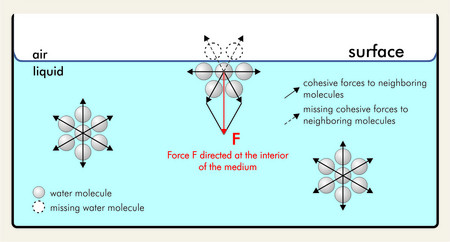
\includegraphics[width=0.6\textwidth]{archivos/surface_tension.png}
	\caption[Caption for LOF]{Illustration of the cohesive forces that result in the surface tension\protect\footnotemark~\cite{sita-process}}
	\label{surface_tension}
\end{figure}

\footnotetext{As it is explained later in this section, this figure is incomplete.}

Within the liquid bulk, a molecule is subject to cohesion forces upon its neighboring particles. They completely surround it resulting in a force equilibrium on that molecule.

Nevertheless, when a molecule belongs to a surface, this symmetry is broken and so does the equilibrium, leading to an increase of the free energy.

But then, 

\begin{displayquote}
	\textit{Why is surface tension a force parallel to the interface while it is so obvious that it must be perpendicular to it?}
\end{displayquote}

This question can be found in Marchand et al.~\cite{Marchand}. Also provided in the aforementioned article is this short answer:

\begin{displayquote}
	\textit{The schematic of Fig. \ref{surface_tension} represents only the attractive intermolecular forces. The real force balance requires both repulsive and attractive interactions between liquid molecules.}
\end{displayquote}

as well as an exhaustive explanation that we will not detail in this document.  

On a more practical level, E\"{o}tv\"{o}s rule allows us to calculate the approximate value of a liquid's surface tension, $\gamma$, as:

\begin{equation} 
\gamma V_m^{2/3}=k\left(T_{c}-T-6\right)
\label{eotvos}
\end{equation}

where $V_m$ is the molar volume, $T_c$ is the critical temperature of the liquid, and $k$ is the Eötvös constant. It has a value of $2.1\cdot 10^{-7} \; \frac{\textrm{J}}{\textrm{K} \cdot \textrm{mol}^{\textrm{2/3}}}$ no matter the liquid.

The resulting value for water at $25^\textrm{o} \textrm{C}$ is $7.17 \cdot 10^{-2} \; \textrm{N/m}$.

\subsubsection{Capillary pressure}

The \textbf{capillary pressure} between two immiscible fluids is defined as:

\begin{equation} 
	p_c = p_{nw} - p_{w}
	\label{cap_pressure}
\end{equation}

where $nw$ and $w$ stand respectively for the non-wetting and wetting phases, meaning $P_c$ represents a pressure jump across the interface. Throughout this section our wetting liquid will be water and the air will be the non-wetting phase. This combination has been extensively studied due to its countless applications.

We will consider that the ambient pressure is known, so we can use equation \ref{cap_pressure} to calculate the pressure on liquid side of the interface. However, we first need the value of the capillary pressure, which is given by the Young-Laplace equation:

\begin{equation} 
p_c = -\gamma \nabla \cdot \hat{n} = 2 \gamma H
\label{young_laplace}
\end{equation}

$H$ being the mean curvature (average of the principal curvatures) of the free surface:

\begin{equation} 
2H = \frac{1}{R_1} + \frac{1}{R_2}
\label{curvature}
\end{equation}

\subsection{Shape of the interface: energetic considerations}

Looking through the literature we found some descriptions of the real shape of the liquid-air interface in contact with a solid wall. 

Generally, two different cases are considered: either the gravity plays an important role or it does not.

An analytic description of the shape resulting of the balance between gravitation and the Young-Laplace pressure drop at the curved surface can be found in the book \textit{Statistical Thermodynamics of Surfaces, Interfaces, and Membranes} by Safran~\cite{Safran}.

When it comes to assessing the case where gravitational forces are negligible, and given there are no other forces, the Young-Laplace pressure drop has to be constant in all the surface. This is because, in a static equilibrium situation, the pressure within the bulk of the liquid has to be uniform. Moreover, if boundary conditions are symmetric with respect to an axis, the shape of the meniscus will hold the same symmetry. 

In his paper, Princen~\cite{PRINCEN1970} calculates the shape and size of the cross section of \textit{Liquid Columns between Horizontal Parallel Cylinders}. For the pressure drop to be uniform, and since one of the radius of curvature is infinite, the other one has to be constant. Therefore, the shape of the free surface is a right circular cylinder.

\begin{figure}[H]
	\centering
	\includegraphics[width=0.3\textwidth]{archivos/drop_column.png}
	\caption{Cross section of a liquid column between two horizontal rods} 
	\label{drop_column}
\end{figure}

To find the value of $R$, the energetic balance proposed by Princen (see Eqs. \ref{princen_eq}) confronts the \textit{free energy $dF$ associated with injecting an infinitesimal volume dV (e.g., from a hypodermic syringe) into the liquid column} with the \textit{work $dW$ done on the system (including the syringe) as a result of the pressure difference across the piston}.

\begin{equation}
\begin{aligned} &\mathrm{d} F=[(AB+CD)-(AC+BD) \cos \theta_0 ] \gamma \mathrm{d} L \\
& \mathrm{d} W= p_c \mathrm{d} V=-\gamma A_{cs} \mathrm{d} L / R \end{aligned}
\label{princen_eq}
\end{equation}

where $A_{cs}$ is the cross-sectional area of the water column.

For such a case, the further addition of liquid does not change the cross section, but only the length of the column. Our geometry, on the contrary, sees its cross area unavoidably dilated because its length is fixed.

This is why we still want to consider another approach: we consider a layer, whose surface is described by the Monge representation (i.e. $h=f(x,y)$ is $Z$ the position of the surface). The free energy of the water-air interface is\footnote{In this section, $h_q$ is the partial derivative of $h$ with respect to the variable $q$, and $h_{qq}$ is the second partial derivative.}:

\begin{equation}
F_{s}=\int \int d x d y\left[\gamma \sqrt{1+h_{x}^{2}+h_{y}^{2}}\right]
\end{equation}

We ignore the energy of the surface between the solid and the wetting phase, assuming that it is negligible since its surface is much smaller. 

To be able to solve it analytically, we are going to consider a circular film instead of a square shaped one. In that case, the orders of magnitude of the aforementioned energies are: 

\begin{equation}
\left\{
\begin{aligned} & F_{air-liquid} = \gamma s_{air-liquid} \sim \gamma \times 2 \times \pi R^2 \sim 4 \cdot 10^{-6} \; \textrm{J} \\
& F_{solid-liquid} = \gamma s_{solid-liquid} \cos \theta  < \gamma \times 2 \pi R \times \pi \rho \sim 1 \cdot 10^{-7} \; \textrm{J}
\end{aligned}
\right.
\end{equation}

where $s_{air-liquid}$ and $s_{solid-liquid}$ are the areas of both interfaces, $R = 3 \; \textrm{mm}$ is the radius of the film, $\rho = 25 \; \mu \textrm{m}$ is the radius of the surrounding thread, and $\theta = 70^\textrm{o}$ is the contact angle between water and nylon. In conclusion, neglecting $F_{solid-liquid}$ seems to be a rather good approximation.

We are now going to minimize the free energy under the constraint of fixed volume using the Euler-Lagrange equation (see Eq. \ref{EulerLagrange}) with a Lagrange multiplier, $\lambda$. The function to minimize is:

\begin{equation}
G=2 \pi \gamma \int_{0}^{R} r\left(1+h_r^{2}\right)^{1 / 2} d r-\lambda 2 \pi \int_{0}^{R} r h d r
\end{equation}

And the Euler-Lagrange equation reads:

\begin{equation}
\frac{\partial f}{\partial h} - \frac{d}{d r}\left(\frac{\partial f}{\partial h_r}\right) = 0
\end{equation}

where, in this case:

\begin{equation}
f\left(h, h_r, r\right)=\gamma r\left(1+h_r^2\right)^{1 / 2}-\lambda r h
\label{EulerLagrange}
\end{equation}

We can now calculate both terms:

\begin{equation}
\left\{\begin{array}{l}{\frac{\partial f}{\partial h}=\lambda r} \\ {\frac{\partial f}{\partial h_r}=\gamma r \frac{h_r}{\left(1+h_r^2\right)^{1/2}} \rightarrow \frac{d}{d r}\left(\frac{\partial f}{\partial h_r}\right)=\gamma\left[\frac{h_r}{\left(1+h_r^{2}\right)^{1/2}}+\frac{r h_{rr}}{\left(1+h^{2}\right)^{1 / 2}}-\frac{r h_r^{2} h_{rr}}{\left(1+h_r^{2}\right)^{3 / 2}}\right]}\end{array}\right.
\label{TermsEL}
\end{equation}

However, before inserting them in Eq. \ref{EulerLagrange}, we need to recall that our Young-Laplace pressure jump must be constant in the whole surface, which leads to the following constraint:

\begin{equation}
\frac{h_{rr}}{\left(1+h_r^{2}\right)^{3 / 2}}-\frac{\sin \left(\operatorname{atan}\left(h_r\right)\right)}{r}=C
\label{PressureConstraint}
\end{equation}

where $C$ is a constant.

We can now simplify the terms in \ref{TermsEL} with the help of \ref{PressureConstraint} and insert them in Eq. \ref{EulerLagrange}, which leads to:

\begin{equation}
h_r=\frac{\frac{1}{2}\left(\frac{\lambda}{\gamma}-C\right) r}{\sqrt{1-\frac{1}{4}\left(\frac{\lambda}{\gamma}-C\right)^{2} r^{2}}}
\end{equation}

In this equation we notice, that, as a consequence of axial symmetry and continuity, the derivative goes to zero when $r$ goes to zero. From now on, we will use the letter $B$ to express the constant $\frac{1}{2}\left(\frac{\lambda}{\gamma}-C\right) R$. Integration of the expression above leads to:

\begin{equation}
h_r=\frac{B \frac{r}{R}}{\sqrt{1-B^{2} \left(\frac{r}{R}\right)^2}} \rightarrow h=-\frac{\sqrt{1-B^{2} \left(\frac{r}{R}\right)^2}}{B} R + K
\end{equation}

where $K$ is a constant.

To find our constants we need to impose the corresponding constraints. The constraint over the volume can be replaced with another determining the value of $h$ in the center of the film, where we want $h$ to be half of the desired thickness:

\begin{equation}
h(r=0) = \frac{t}{2} = h_0 \rightarrow K = \frac{R}{B} + h_0
\end{equation}

\begin{figure}[H]
	\centering
	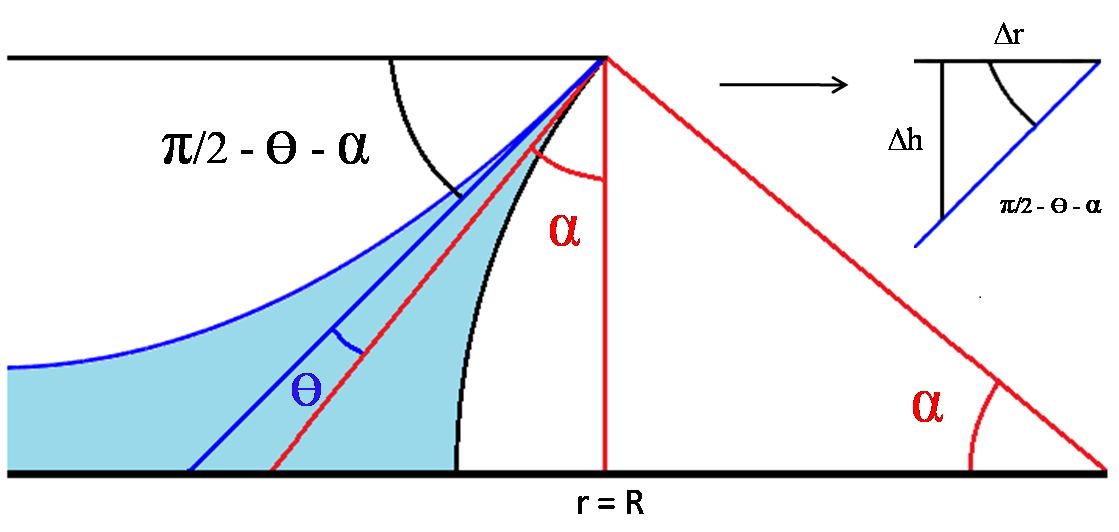
\includegraphics[width=0.7\textwidth]{archivos/geom_film.png}
	\caption{Diagram of a the liquid film next to the thread.}
	\label{geom_film}
\end{figure}

The second constraint is the contact angle between the liquid and the solid. Fig. \ref{geom_film} helps us find out the expression of this constraint:

\begin{equation}
h_r(r=R)=\tan \left(\frac{\pi}{2}-\theta-\alpha\right) 
\end{equation}

where $\alpha=\textrm{asin} \left[\frac{h(r=R)}{\rho}\right]$. This leads to:

\begin{equation}
\tan[(\operatorname{asin}[B])] = \tan \left[[\frac{\pi}{2}-\theta-\operatorname{asin}\left(-\frac{\sqrt{1-B^{2}}}{B} \frac{R}{\rho}+\frac{1}{B}\frac{R}{\rho}+\frac{h_0}{\rho}\right)\right]
\end{equation}

Since $\|B\|$ has to be smaller than one for it to have a solution, this equation can be rewritten as:

\begin{equation}
\sin \left(\frac{\pi}{2} - \theta \right) (1 - B^2)^{1/2} B - \cos \left(\frac{\pi}{2} - \theta\right) B^2 = - [(1 - B^2)^{1/2}+1] \frac{R}{\rho} + \frac{h_0}{\rho} B
\end{equation}

For the values $R = 3 \; \textrm{mm}$, $\rho = 25 \; \mu \textrm{m}$ and $\theta = 70^\textrm{o}$, $h_0 = t/2 = 7.5 \; \mu \textrm{m}$, which are similar to the dimensions of our film, we obtain $B \simeq 6.90 \cdot 10^{-4}$ and a volume of $ \simeq 0.45 \; \mu \textrm{L}$. The shape of the film is shown in the next figures:

\begin{figure}[H]
	\centering
	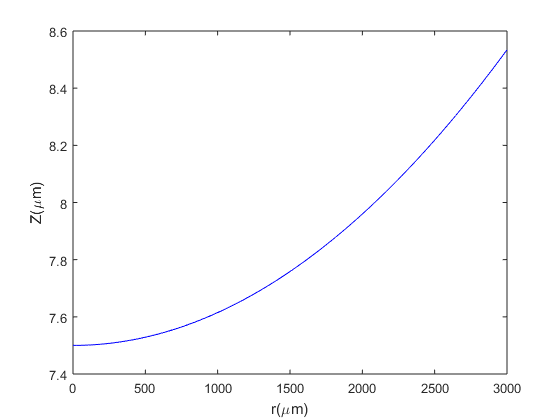
\includegraphics[width=0.6\textwidth]{archivos/CircFilmFunction.png}
	\caption{Half thickness of the film as a function of the radial position.}
	\label{CircFilmFunction}
\end{figure}

\begin{figure}[H]
	\centering
	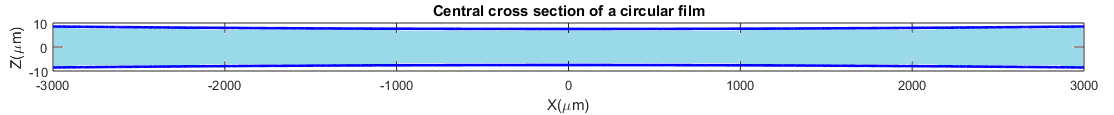
\includegraphics[width=\textwidth]{archivos/CircFilmSection.png}
	\caption{Diagram of a the liquid film next to the thread.}
	\label{CircFilmSection}
\end{figure}

Far enough from the boundary conditions we can expect a similar shape for a square shaped film, so indeed we can consider that it is mostly flat.

\section{Surfactants}

A surfactant is a chemical substance that, when used as a solute, reduces the surface tension of the colloid. Hence, they are also called surface-active agents.
 
Surfactant molecules have at least one portion of their structure that is hydrophobic and one part that is hydrophilic. It is this duality that gives them their unique properties.
 
These substances reduce the surface tension of their solvent by acting like an inter-phasial bridges between the fluid and the air. In fluids like water the hydrophilic portion of the molecule will orient itself towards the fluid, while the hydrophobic portion will point outwards. This accommodation reduces the total amount of energy needed in to form the surface of the fluid, thus reducing the surface tension.
 
Surfactants may also form aggregates, normally spherical, called micelles. In this assemblies of molecules, the hydrophilic parts form the outer layer of the sphere while the hydrophobic groups point inwards avoiding direct contact with the solvent.

\section{Flowing films}

As we will see later, in the ¿¿¿Results and Analysis??? section, flows unrelated to algae motion (what we call \textit{background flows}) have been an important issue in this research.

To understand them, we looked for bibliography on several topics, among which, flowing films (see Fig. \ref{flowing_film}).

We developed some equations for our problem (quasi-horizontal layer) based on Rutgers' 2D model ¿¿¿ Rutgers 1998 ??? of a falling vertical film. This model an air box of width L through and thickness 2d around the film and calculates both the velocity field in the air and the film. Motion is not driven, as usual, by a pressure gradient, but by the force of gravity on the film.

\begin{figure}[H]
	\centering
	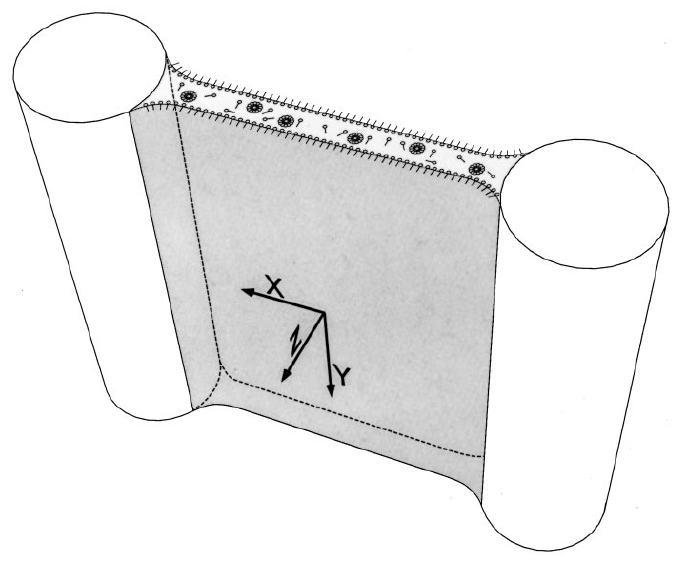
\includegraphics[width=0.4\textwidth]{archivos/FilmBetweenWires.png}
	\caption{Diagram of a liquid film between two wires~\cite{Rutgers2001}. The \textit{head and tail} structures represent molecules of surfactant.}
	\label{flowing_film}
\end{figure}

This model constitutes a very simplified approach, because it is obvious that our boundary conditions are going to have an important effect (i.e. our fluid is never renewed, but it recirculates), but it should at least give us an idea of the magnitudes in our problem.

The equation for the surrounding air reads :

\begin{equation}
\frac{\partial^{2} v_{\mathrm{a}}(x, z)}{\partial x^{2}}+\frac{\partial^{2} v_{\mathrm{a}}(x, z)}{\partial z^{2}}=0
\label{air_velocity}
\end{equation}

And the one for the film itself:

\begin{equation}
\mu_{2D} \frac{d^{2} v(x)}{d x^{2}}=-2 \mu_{\mathrm{a}}\left|\frac{\partial v_{a}(x, z)}{\partial z}\right|_{z=0^{+}}-\rho h g \sin \alpha
\label{film_velocity}
\end{equation}

where $v_{\mathrm{a}}$ velocity on the film (i.e. at $z = 0$), $h$ is the thickness of the film and $\mu_{2D}$ is a 2D viscosity that we will address more specifically later. The second term of the right side results from the continuity of tangential efforts at the interfaces.

As for the the boundary conditions:

\begin{equation}
\left\{
\begin{aligned}
& v(x=0) = 0 \quad \text{(No slip on the wire)} \\
& dv/dx(x=L/2) = 0 \quad \text{(Symmetry)} \\
& v_{\mathrm{a}}(x,z=0^+) = v(x) \quad \forall x \quad \text{(No slip on the interface)}\\
& dv_{\mathrm{a}}/dx(x=L/2,z) = 0 \quad \text{(Symmetry)} \\
& v_{\mathrm{a}}(x=0,z) = 0 \quad \text{(No slip on the wall\protect\footnotemark)} \\
& v_{\mathrm{a}}(x \rightarrow \infty,z) = 0 \quad \text{(Ambient conditions)}
\end{aligned}
\right.
\end{equation}

\footnotetext{After validating its negligible effect experimentally, ¿¿¿ Rutgers et al.??? confine their film between two glass plates.}


%IVANOV:
% Critical thickness of film rupture: According to Scheludko (14) the rupture of thin films is due to thermal fluctuations which lead to corragation of the film surface. The shape of the surface at any moment can be presented as a superposition of an infinite number of fluctuation waves with various lengths and amplitudes. Let us suppose for simplicity that there is only one wave with wave-number k_n.The vertical displacement of the film surface at a given point from its position in the absence of waves (i.e. in a plane-parallel film) we shall denote by \zeta_n.

%We shall only consider the case of symmetrically situated waves which are responsible for the rupture(16). Thus the local film  thickness will be h+2 \zeta_n. For simplicity we  shall assume that the wave has a cylindrical  symmetry.
			
%The corrugation of the surface give rise to  two forces: the first one caused by the local  capillary pressure tends to smooth the film  surface while the second one due to the increase  of the negative disjoining pressure (with respect  to its value in the plane-parallel film), tends to  increase \zeta_n. If h is large the first effect prevails,  if it is small the second one, so that for a given wave a transition thickness  h_0 exists at which the  character of wave motion changes. While at h>h_0 the surface performs oscillations around  the equilibrium position  \zeta_n=0, at h<h_0 the  oscillations cease and liquid is transfered continously into the thicker parts of the film. Thus \zeta_n continuously grows until the film breaks or a black spot is formed (14). 

	\section{Active suspensions}
\label{active_suspensions}

Active suspensions are densely packed soft materials whose constituents can self-propel.

In turn, soft materials~\cite{Soft_materials} are those that can be easily deformed by external stresses, electric or magnetic fields, or by thermal fluctuations. 

As Pierre-Gilles de Gennes said during his Nobel Prize lecture~\cite{PGG}, another designation for these materials is \textit{complex fluids}, which renders very well their complex and flexible character.

They are considered 'structured fluids' because they have the local mobility of ordinary fluids, but they always show a degree of local order (see~\cite{soft_matter},~\cite{Hamley}).

In particular, we will be working with biological soft materials\footnote{In the introduction we mentioned the existence of synthetic active suspensions. For the sake of brevity, they remain out of the scope of this document. If the reader is curious about this topic, further information can be found, for instance, in the paper of Thutupalli et al.~\cite{Thutupalli}, who experimentally studied the behavior of droplets displacing under Marangoni stresses.} which may, or not, be amphiphile \footnote{Surfactants are amphiphilic compounds: they possess both hydrophilic and hydrophobic moieties (head and tail respectively).} solutions as well.

Contrary to many other soft materials, the presence of \textit{Chlamydomonas reinhardtii} does not seem to affect the \textbf{rheological properties} of water significantly (i.e. it stays a Newtonian fluid with a very similar viscosity coefficient). Surfactants may, on the other hand, change some of these properties in a local way, mainly at the surfaces (where they are mostly concentrated), as a consequence of the Marangoni effect.

It is though clear that \textbf{diffusion} is modified (enhanced) by the action of \textit{Chlamydomonas reinhardtii}, so the sections hereafter are devoted to biological and physical aspects of this alga.

\subsection{\textit{Chlamydomonas reinhardtii}}
\label{chlamy}

\subsubsection{Classification and biological description}
\label{bio_chlamy}

We have already mentioned that \textit{Chlamydomonas reinhardtii}
is a unicellular green alga, but we would like to provide with a more exhaustive description through its taxonomic classification: 

\begin{itemize}
	\item \textbf{Superregnum}: Eukaryota - Organisms whose cells have a nucleus enclosed within membranes	
	\item \textbf{Regnum}: Plantae/Viridiplantae - Clade made up of the green algae, which are primarily aquatic, and the land plants
	\item \textbf{Divisio}: Chlorophyta - Division of the green algae that comprises about 8200 species, the majority of whom are aquatic and photosynthetic
	\item \textbf{Classis}: Chlorophyceae - One of the classes of green algae, distinguished mainly on the basis of ultrastructural\footnote{Ultrastructure is the architecture of cells and biomaterials that is visible at higher magnifications than found on a standard optical light microscope (e.g.: organelles)} morphology
	\item \textbf{Ordo}: Volvocales/Chlamydomonadales~\cite{chlorophyceae} - Members of these orders have a 1 o'clock-7 o'clock arrangement of the basal bodies of the flagella.
	\item \textbf{Familia}: Chlamydomonadaceae - This family includes all the unicellular Volvocales. They may be bi- or quadriflagellate.
	\item \textbf{Genus}: Chlamydomonas\footnote{For further information on the genus Chlamydomonas we recommend the book of Pandey~\cite{Pandey}} - Species of this genus have a cell wall, a single chloroplast, an eye-like structure for sensing light and two anterior flagella used for displacement, generally through a breast-stroke type motion.
	Scientists have described over 500 species in this genus and a few of its species are widely used as model organisms.
	https://www.chlamycollection.org/resources/about-chlamydomonas/
	\item \textbf{Species}: Chlamydomonas reinhardtii - according to Pröschold et al.~\cite{Proschold}, all the current “standard” \textit{C. reinhardtii} strains are presumably derived from a single field-isolated zygote in Massachusetts in 1945\footnote{For detailed information, both the article od Pröschold et al. and the one of Harris~\cite{Harris} should be consulted.}. Its diameter is about 10 micrometres; it has a cell wall, a large cup-shaped chloroplast, and an "eyespot" that senses light. 
\end{itemize}

The figure below shows a schematic of the cross section of \textit{C. reinhardtii}:

\begin{figure}[H]
	\centering
	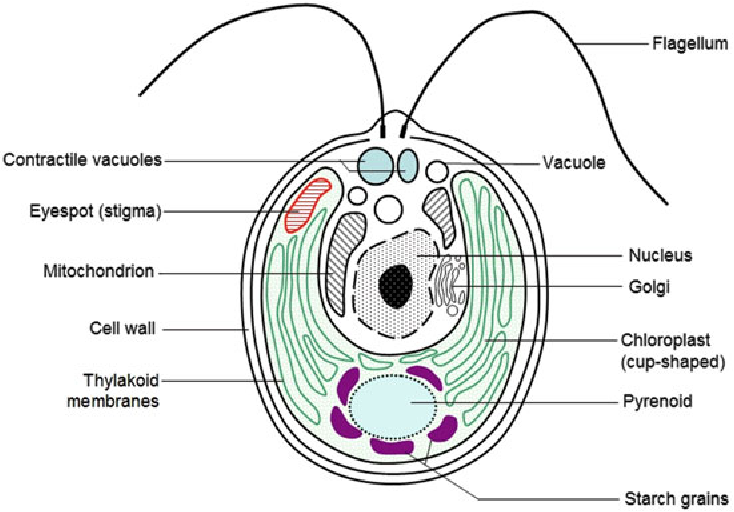
\includegraphics[width=0.8\textwidth]{archivos/chlamy_illustration.png}
	\caption{Schematic of \textit{C. reinhardtii} cross section~\cite{chlamy_cs}
	}
	\label{chlamy_illustration}
\end{figure}

Especially important to our research is the motion of this alga and its mechanisms. A more mechanical point of view will be adopted in the next section, but we consider it important to explain some phenomena that could modify the motion patterns of \textit{C. reinhardtii}. Originated in response to a stimulus, this movements are referred to as taxes. Depending on the cause they are classified as: aerotaxis (stimulation by oxygen), barotaxis (by pressure), chemotaxis (by chemicals), galvanotaxis (by electric current), gravitaxis (by gravity), hydrotaxis (by moisture), magnetotaxis (by magnetic field), phototaxis (by light), rheotaxis (by fluid flow), thermotaxis (by changes in temperature), thigmotaxis (by physical contact)...

\subsubsection{Physical description and modelisation}
\label{phys_chlamy}

The study of the motion of microorganisms (microswimmers) in an analytical way was first addressed by Lighthill in 1952~\cite{Lighthill}. He developed the \textit{spherical squirmer model}, which considers the microorgnism as a spherically shaped particle that uses small-amplitude, axisymmetric surface distortions to move through the surrounding fluid.

Still today, the spherical squirmer is widely used as a model for self-propelled particles, such as unicellular protists, algae, Janus particles\footnote{Janus particles are entities whose surface shows different functionalities on different parts of it~\cite{PGG}.}, etc. in Stokes flow.

Later, in 1971, Lighthill’s student John Blake,  corrected and refined Lighthill's theory. This model tackled ciliated organisms and involved the behavior of the envelope covering the end of that cilia. 

\begin{figure}[H]
	\centering
	\includegraphics[width=0.6\textwidth]{archivos/BlakeWave.PNG}
	\caption[Caption for LOF]{Envelope showing a symplectic metachronal wave\protect\footnotemark ($---$)~\cite{Pedley}}
	\label{symplectic_wave}
\end{figure}

As it can be seen on the previous figure, the cilia take on asymmetric conformations to overcome the time reversibility of Stokes flows: during the power stroke they are mostly stretched and during the recovery strokes they remain contracted.

Regarding the spherical simplification, in Blake's own words: \textit{Considering the problem of a sphere is highly idealizing the shape of the organism, but at low Reynolds number the shape does not alter the hydrodynamical features very greatly.} With the right coordinate transformation, other shapes could be considered, but it would add nothing new beyond making the calculations more obscure.

\footnotetext{A phase difference between the flagella leads to the generation of a metachronal wave. A negative phase difference creates symplectic waves (i.e. the direction of beat and wave transmission is the same) due to compression of the cilia during the effective stroke phase. A positive phase difference results in antiplectic waves (i.e. the directions of beat and wave transmission are opposed) by compression on the cilia during the recovery stroke.}

In the considered case (low $Re$, incompressible, axisymmetric flow), the equations of motion for the velocity $\mathbf{u}$ and pressure $p$ are: 

\begin{equation}
\begin{aligned} & \nabla \cdot \mathbf{u}=0 \\
& \nabla p-\mu \nabla^{2} \mathbf{u}=\mathbf{F} \label{stokes_f} \end{aligned}
\end{equation}

It is clear, that, due mainly to its tiny size and relatively low speed, microorganisms live in the world of low Reynolds number. However, for this equations to be suitable, another condition must be accomplished since swimming flows are usually unsteady: the ‘frequency Reynolds number’ $Sr \cdot Re = \rho \omega l_c^2/ \mu_g$ (where $Sr$ is the Strouhal number) must also be small.

In our problem the value of both Reynolds numbers can be estimated as follows:

\begin{equation}
	\begin{aligned} & Re = \rho_g u_c l_c/\mu_g \simeq 1.32 \cdot 10^{-4} << 1\\
	& Sr \cdot Re = \rho_g \omega_cl_c^2/ \mu_g \simeq 4.96 \cdot 10^{-4} << 1 \end{aligned}
\end{equation}

as $\rho_p = 1.05 \; \textrm{g/} \textrm{cm}^\textrm{3}$, $l_c = 1 \; \mu \textrm{m}$,  $u_c = 100 \; \mu \textrm{m/s}$,  $\omega_c = 2 \pi 60 \; \textrm{rad/s}$, and we consider the worst-case scenario regarding the temperature: $\mu_g(30^\textrm{o}\textrm{C}) = 7.98 \cdot 10^{-4} \; \textrm{kg/(m} \cdot \textrm{s)}$

These values widely justify the use of the Stokes equations in this context.

A very interesting interpretation of the Reynolds number is provided by Lauga and Powers in their 2009 article on \textit{The hydrodynamics of swimming microorganisms}~\cite{Lauga}. The Reynolds number would compare the time scales for the convective transport of a local velocity perturbation along the body ($t_{adv} \sim l_c/u_c$), and for viscosity to diffuse this perturbation  away from the body ($t_{diff} \sim ρl_c^2/ \mu_g$). 

As a consequence, in low Reynolds number flows, velocity perturbations diffuse before being carried along by the flow and thus the response of the fluid to the displacement of its boundaries must be immediate. 

In conclusion, the acceleration of a microswimmer is negligible as against the forces from the surrounding fluid. As a result of this absence of inertia, Newton’s law becomes:

\begin{equation}
\mathbf{F_{\mathrm{ext}}}(t)+\mathbf{F}(t)= \mathbf{0}
\end{equation}

which constitutes an instantaneous balance between external and fluid forces \footnote{A similar result can be found regarding the torques, but we will not make use of it in this document.}.

Consequently, in absence of external forces $\mathbf{F}(t) = \mathbf{0}$. This obviously requires a density matching of the swimmers and the medium.

Equations \ref{stokes_f} become then:

\begin{equation}
\begin{aligned} & \nabla \cdot \mathbf{u}=0 \\
& \nabla p-\mu \nabla^{2} \mathbf{u}=\mathbf{0} \label{stokes_f} \end{aligned}
\end{equation}

Since only motions with axial symmetry are considered, spherical polar co-ordinates represent a logical choice. With a moving origin that remains at the center of the body \footnote{Lighthill justifies neglecting any inertial translation this origin may undergo because: \textit{This motion of the origin makes no difference to the equations of motion, since the inertial force associated with it is clearly equally negligible with those already neglected.}}, the solution in terms of radial and azimuthal velocities $u_r$ and $u_\theta$ presented by Blake~\cite{Blake} is:

\begin{equation}
\begin{aligned} u_{r}\left(r, \theta_{0}\right)=&-U \cos \theta_{0}+A_{0} \frac{a^{2}}{r^{2}} P_{0}+\frac{2}{3}\left(A_{1}+B_{1}\right) \frac{a^{3}}{r^{3}} P_{1} \\ &+\sum_{n=2}^{\infty}\left[\left(\frac{1}{2} n \frac{a^{n}}{r^{n}}-\left(\frac{1}{2} n-1\right) \frac{a^{n+2}}{r^{n+2}}\right) A_{n} P_{n}+\left(\frac{a^{n+2}}{r^{n+2}}-\frac{a^{n}}{r^{n}}\right) B_{n} P_{n}\right] \\ u_{\theta}\left(r, \theta_{0}\right)=& U \sin \theta_{0}+\frac{1}{3}\left(A_{1}+B_{1}\right) \frac{a^{3}}{r^{3}} V_{1} \\+& \sum_{n=2}^{\infty}\left[\left(\frac{1}{2} n \frac{a^{n+2}}{r^{n+2}}-\left(\frac{1}{2} n-1\right) \frac{a^{n}}{r^{n}}\right) B_{n} V_{n}+\frac{1}{2} n\left(\frac{1}{2} n-1\right)\left(\frac{a^{n}}{r^{n}}-\frac{a^{n+2}}{r^{n+2}}\right) A_{n} V_{n}\right] \end{aligned}
\label{stokes_sol_uv}
\end{equation}

where $a$ is the radius of the spherical squirmer, $B_n$ are constant coefficients, $P_n(cos \theta)$ are Legendre polynomials\footnote{Solutions to the Legendre Differential Equation, whose form is:\\ $P_{n}(x)=\sum_{m=0}^{M}(-1)^{m} \frac{(2 n-2 m) !}{2^{n} m !(n-m) !(n-2 m) !} x^{n-2 m}$ with \\ $M=n / 2$ or $(n-1) / 2,$ whichever is an integer} and:

\begin{equation}
V_{n}(\cos \theta)=\frac{2}{n(n+1)} P^1_{n}(\cos \theta)
\end{equation}

where $P^1_n$ is the associated Legendre function of the first kind\footnote{The defining relationship between Legendre functions (of order $m$) and Legendre polynomials is: $P_{n}^{m}(x)=\left(1-x^{2}\right)^{m / 2} \frac{d^{m} P_{n}(x)}{d x^{m}}$}.

The coefficients of \ref{stokes_sol_uv} correspond to the sole solution that fulfills the boundary conditions at the surface\footnote{The boundary conditions are given at $r=a$ because the amplitude of the perturbations is much smaller than $a$} of the squirmer:

\begin{equation}
u_r|_{r-a}=\sum_{0}^{\infty} A_{n} P_{n}, \quad u_\theta|_{r-a}=\sum_{0}^{\infty} B_{n} V_{n}
\end{equation}

Among the fundamental solutions that conform \ref{stokes_sol_uv} we must only retain those which represent motions with a finite total energy (infinite energy solutions can only arise of the continued application of an external force). As a consequence, to avoid infinite terms resulting from the integration leading to the system's energy, the velocity of the origin must be:

\begin{equation}
	U=\frac{1}{3}\left(2 B_{1}-A_{1}\right)
	\label{deformation_vel}
\end{equation}

This condition also requires to omit the \textbf{Stokeslet} term ($\propto r^{-1}$ in 3D) in both expressions (it has been already omitted in Eqs.\ref{stokes_sol_uv}), meaning that the Stresslet solution ($\propto r^{-2}$ in 3D)\footnote{Stresslets are obtained by differentiation of the Stokeslets and, thus, their spatial decay is faster.} will dominate the field.

With the aim of illustrating the fundamental solutions to the Stokes equation, Fig. \ref{stokeslet_stresslet} shows the velocity field corresponding to a Stokeslet and a Stresslet in 3D.

\begin{figure}[H]
	\centering
	\includegraphics[width=0.8\textwidth]{archivos/stokesletstresslet.jpg}
	\caption{Velocity field around a Stokeslet (left) and around a Stresslet (left)~\cite{Singh2015}. Streamlines are overlaid on a pseudocolor plot of the logarithm of the magnitude of the fluid velocity in a planes containing the axis of the symmetry}
	\label{stokeslet_stresslet}
\end{figure}

Another point of view that would equally lead us to omit the Stokeslet term is the fact that these solutions are associated with singular point forces, which, as we have already explained, are not present in this problem. 

The given explanation, however, is not trivial and it can help to look at a smaller scale of our specific problem, where one can consider two Stokelet fields that somehow compensate each other: the flagellar thrust and the body drag~\cite{Lokenath}. In their 2018 paper~\cite{Drescher2010}, Drescher et al. develop a three-Stokeslet model that illustrates this thrust-drag balance (see Fig. \ref{drag_thrust}).

\begin{figure}[H]
	\centering
	\includegraphics[width=0.7\textwidth]{archivos/velfield.png}
	\caption{Time- and azimuthally- averaged flow field of \textit{C. reinhardtii}. (a) Streamlines (red) computed from velocity vectors (blue). The spiraling near elliptic points is an artifact of the direct integration a noisy experimental velocity field. A color scheme indicates flow speed magnitudes. (b) Streamlines of the azimuthally averaged flow of the three-Stokeslet model: flagellar thrust is distributed among two Stokeslets placed (not fitted) at the approximate flagellar position (lateral green arrows), whose sum balances drag on the cell body (central red arrow)~\cite{Drescher2010}.}
	\label{drag_thrust}
\end{figure}

Finally one can derive an expression for the pressure:

\begin{equation}
p=\mu_{n=2}^{\infty} \frac{2 n-1}{n+1}\left(n A_{n}-2 B_{n}\right) \frac{a^{n}}{r^{n+1}} P_{n}\left(\cos \theta_{0}\right)
\end{equation}

The fact that flagella and cilia, although similar, show some important differences cannot be ignored. Nonetheless, the squirmer model remains applicable.

Extensions to ellipsoidal swimmers and time-dependent swimming gaits for a reduced squirmer model are explained in Delmotte  et al.~\cite{Delmotte2015}. Although the time-averaged models (e.g.: squirmer model with constant coefficients) provide with valid results for the far field, the experimental works of Guasto et al.~\cite{Guasto} suggest that time dependence has, in fact, an important effect on the close field of a swimmer. This must be taken into account when working with high swimmer concentrations.

The reduced model used by Delmotte is proposed by Ishikawa et al. in~\cite{Ishikawa}. It considers $A_n=0$ for all $n$ and $B_n=0$ for all $n >2$. The resulting flow field in the moving frame attached to the swimmer is:

\begin{equation}
\begin{array}{l}{\mathbf{u}_{\Gamma}(r, \theta)=\frac{2}{3} B_{1} \frac{a^{3}}{r^{3}} P_{1}(\cos \theta)+\left(\frac{a^{4}}{r^{4}}-\frac{a^{2}}{r^{2}}\right) B_{2} P_{2}(\cos \theta)} \\ {\mathbf{u}_{\theta}(r, \theta)=\frac{1}{3} B_{1} \frac{a^{3}}{r^{3}} V_{1}(\cos \theta)+\frac{a^{4}}{r^{4}} B_{2} V_{2}(\cos \theta)}\end{array}
\end{equation}

In the absence of $A_1$, Eq. \ref{deformation_vel} shows that the first mode and, thus, $B_1$ is directly related to the swimming speed. It can also be shown [28] that the second mode and its coefficient, $B_2$, are directly related to the Stresslet. 

A parameter $\beta=B_2/B_1$ can now be introduced that describes the relative Stresslet strength and allows us to distinguish two sorts of mechanisms: when $\beta>0$, the squirmer behaves like a \textit{puller}, bringing fluid in along its swimming direction and expelling it laterally; otherwise ($\beta<0$), the squirmer acts like a \textit{pusher}, expelling fluid along  its swimming direction and bringing it in laterally. Examples of the flow patterns induced by this two types of microswimmers can be observed in Fig. \ref{push_pull}.

\begin{figure}[H]
	\centering
	\includegraphics[width=0.6\textwidth]{archivos/push_pull.png}
	\caption{Schematics showing the flow patterns induced by classical (a) pushers (\textit{Escherichia coli}) and (b) pullers (\textit{Chlamydomonas reinhardtii}). The color indicates the magnitude of the flow ($r^{−2}$ scaling because of the dominating Stresslet).~\cite{Yang}}
	\label{push_pull}
\end{figure}

On one hand, \textit{Pushers} and \textit{pullers} show some differences regarding the rheological properties of the suspension they are immersed in: the effective viscosity is increased in the case of \textit{pullers} and decreased for \textit{pushers}.

On the other hand, the enhancement of diffusion or mixing has very similar characteristics, that will be discussed in greater depth in the State of the art section. 
	%%%%%%%%%%%%%%%%%%%%%%%%%%%%%%%%%%%%%%%%%%%%%%%%%%%%%%%%%%%%%%%%%%%%%%%%
% Plantilla TFG/TFM
% Escuela Politécnica Superior de la Universidad de Alicante
% Realizado por: Jose Manuel Requena Plens
% Contacto: info@jmrplens.com / Telegram:@jmrplens
%%%%%%%%%%%%%%%%%%%%%%%%%%%%%%%%%%%%%%%%%%%%%%%%%%%%%%%%%%%%%%%%%%%%%%%%

\section{Brownian motion}
\label{brownian}

According to Encyclopedia Britannica~\cite{BritannicaBrownian}, \textit{Brownian motion is any of various physical phenomena in which some quantity is constantly undergoing small, random fluctuations.}

It gets its name from Robert Brown, the Scottish botanist  who studied it in the first place, circa 1827, in the context of microscopic particles within the pollen grains suspended in water under the microscope. Brown himself would dismiss the theory that this motion had a biological origin.

Half a century later, in view of the relationship between temperature and Brownian velocity, it was suggested that this phenomenon could be caused by the thermal molecular motion of environment.

If true, this would be the first directly observable proof of the kinetic theory\footnote{According to the kinetic theory, the temperature of a substance is proportional to the average kinetic energy with which the molecules of the substance are moving or vibrating: $T=\frac{2}{3} \frac{K}{N k_{B}}$, where $N$ is the number of molecules, $K=\frac{1}{2} N m \overline{v}^{2}$ is the kinetic energy of the system, and $k_{B} = 1.380649 \times 10^{-23} \; \textrm{J/K}$ is the Boltzmann constant}, developed in the late 19th century by Maxwell, Boltzmann and Clausius.

In the beginning of the 20th century, Einstein and Smoluchowski separately produced their quantitative theories of Brownian motion. 

A few years later, the verification of Einstein's model by Jean Perrin would finally demonstrate the atomic nature of matter.

\subsection{From Brownian motion to diffusion}

If in a given medium, the random motion of its particles has no preferred direction, then as time passes, the particles will tend to be spread evenly throughout it.

This process can also be interpreted as a subtance spreding from regions of high concentration to regions of lower concentration, and it is called diffusion. Hence, diffusion can be considered an emergent manifestation on a macrospic level of particles subject to Brownian motion on the microscopic level.

Einsten developed a model based on probability theory that shows that the density of Brownian particles $\rho$ at a point $x$ at time t satisfies the diffusion equation: ???

\begin{equation}
\frac{\partial \rho}{\partial t}=D \frac{\partial^{2} \rho}{\partial x^{2}}
\end{equation}

The solution to this equation, assuming a boundary condition were all particles are at the origin at time t=0 is a normal distribution with mean $\mu=0$ and variance $\sigma^{2}=2 D t$.

Given $\mu=0$, it is possible to conclude that  meaning that a Brownian particle is equally likely to move in any sense and direction.

The second moment\footnote{The $n^{th}$ moment of a real-valued continuous function f(x) of a real variable is defined as:  $\mu_{n}=\int_{-\infty}^{\infty} x^{n} f(x) \mathrm{d} x$} of the distrubution is:

\begin{equation}
\overline{x^{2}}=2 D t
\end{equation}

This allowed Einstein to show that the displacement of a Brownian particle is not proportional to the elapsed time, but rather to its square root.

In a state of dynamic equilibrium, established between concentration driven migration and other present forces, the particle density distribution combined with Fick's Law leads to:

\begin{equation}
D=q k_{\mathrm{B}} T
\end{equation}

where $q = \frac{v}{F_ext}$ is the mobility of a particle in the surrounding fluid, which for a spherical particle with radius $r$ is, as Stokes demonstrated: 

\begin{equation}
q=\frac{1}{6 \pi \mu r}
\end{equation}

Thus, a smaller particle, a less viscous fluid, and a higher temperature would each increase the diffusion coefficient and, therefore, the mean square displacement (MSD). 

\subsection{Influence of microswimmers}

In active suspensions, besides the molecular bombardment, the MSD of Brownian particles can be further enlarged through interactions with the active particles. This interaction can be due to either direct contact or simply to their influence on the flow field.

\begin{figure}[H]
	\centering
	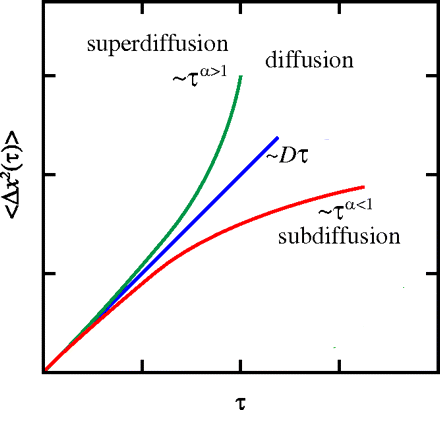
\includegraphics[width=0.4\textwidth]{archivos/SubSuperDif.png}
	\caption{Scaling of the mean square displacement in the scenarios of subdiffusion, diffusion and superdiffusion~\cite{MacKintosh7138} (modified)}
	\label{SSDif}
\end{figure}

Depending on several factors (concentration, elapsed time), the presence of microswimmers can modify the value of the diffusion coefficient (i.e. enlarged gaussian distributions at high concentrations and long times~\cite{Kurtuldu2011}) and even the scaling of the MSD (i.e. modified tails of the distributions at relatively short times~\cite{Kurtuldu2011}). 
	\chapter{State of the art}
\label{SOA}

This section constitutes an extremely brief summary of the latests studies (to our knowledge). For further detail, we recommend the reading of annual reviews on the topic such as the one of Saintillan~\cite{Saintillan}.

\section{Enhancement of diffusion and mixing: pushers and pullers}
\label{SOA_mixing}

The flow fields induced by microorganisms, improve transport and, therefore, mixing in suspensions. The way in which they do that depends, among other things, on their swimming patterns. As we have already stated, isolated swimmers generate different flow fields depending on if they are pullers or pushers. 

Orientation decorrelation mechanisms are as important for mixing as the way of swimming. These mechanisms are mainly of two types: \textit{run-and-tumble} motion and \textit{rotational diffusion}. The former, usually depending on the microswimmers themselves, consists of straight runs that alternate with random tumbles with a certain mean frequency. The latter is a combination of thermal Brownian motion, whose contribution is weak, and other sources of noise such as flagellar beating patterns.

When in groups, the perturbations exerted of the swimmers on the fluid overlap. This can have different effects depending on the level of concentration. Moreover, hydrodynamic interactions that can take place can even lead to coherent motion\footnote{This meso-scale structures have been studied for concentrated bacterial cells, but not for algal cells}, substantially changing the flow field. Interactions between microorganisms have been studied by several authors, among which we would like to cite Ishikawa (~\cite{Ishikawa},~\cite{Ishikawa9}), who, with a bottom-up approach, studied a wide range of possibilities, from interactions between two individuals to a continuum suspension level.

In spite of the apparent differences, several studies on pushers and pullers show that the dynamics of spherical tracers are qualitatively similar in both cases (see, for example, Wu and Libchaber~\cite{Wu} and Leptos et al.~\cite{Leptos}). In 2016, however, Yang et al.~\cite{Yang} would show that ellipsoidal tracers behave differently (in their rotational degree of freedom), depending on the nature of the present active particles, allowing their distinction.

Another important factor is dimensionality: in a 2D confinement such as ours, the pysical model for pushers and pullers explained in section \ref{phys_chlamy} remains valid. However, the dominant solution, a Stresslet, presents a larger field of influence. In 3D the velocity field generated by a Stresslet is $\propto r^{-2}$, whereas in 2D, it is $\propto r^{-1}$. Our reference article on this topic is the one of Kurtuldu et al.~\cite{Kurtuldu2011}, where the 2D environment is limited by free surfaces in order to avoid no-slip conditions. 

\section{Modeling microswimmers: an outline}
\label{SOA_modeling}

An introduction to the analytical approach has already been presented in Section \ref{phys_chlamy}. This section aims to give an insight to the numerical methods, that, based on the analytical ones, allow the analysis of greater systems, different levels of concentration...

Although continuum models are, of course, possible and have been developed (see Toner et al.~\cite{Toner}), the natural choice for the numerical description of active suspensions are particle-based simulations.

Continuum models generally rely on the description of far-field hydrodynamic interactions, which limits their validity to relatively dilute suspensions.

In particle-based simulations, microswimmers are immersed in a continuous medium and the dynamics of each one of them is resolved in a highly coupled system. The description of individual swimmers includes high-order singularities due to particle size (i.e. close-field hydrodynamic interactions), which remain exceptional in the continuum models. The resulting positions and orientations finally allow us to depict the whole dynamics of the suspension.

The choice of the model for individual swimmers can greatly affect the output of the system simulations. Some candidates for modelling the individual behavior are the spherical squirmer model of Lighthil and Blake~\cite{Blake}, slender-body theory~\cite{batchelor_1970} of rod-like swimmers and point force distributions, such as the three-Stokeslets model proposed by Drescher et al.~\cite{Drescher2010}.

Delmotte et al.~\cite{Delmotte2015} have developed a numerical method based on the squirmer model, that has demonstrated great versatility and efficiency, taking into account short range effects such as steric interactions. 

This method \textit{extends the force-coupling method (FCM) to active particles by introducing the regularized singularities in the FCM multipole expansion that have a direct correspondence to the surface velocity modes of the squirmer model}.

In the FCM, the effect of particles on the fluid phase is represented by a localized body force that transmits to the fluid, thus representing an extra term in the Navier-Stokes equations. This force is described by a regularized multipole expansion, whose terms (monopoles, dipoles...) decay with the distance to its source, but do not tend to infinite at the source point (Gaussian shapes are usually chosen). This allows the total particle force, the one associated with constraints included, to be projected onto a structured and simple grid over which an efficient parallel Stokes solver can simultaneously process all the hydrodynamic interactions and eventually find the whole fluid field.

\textbf{Recently, Delmotte et al.~\cite{Delmotte2018} have used this method to perform simulations whose goal is to examine tracer displacements and effective tracer diffusivity in squirmer suspensions. Our experiments are partially aimed at validating the latest upgrade of this model, which consists in simulating free-surface type boundary conditions.}



	\chapter{Materials and methods}
\label{materias_methods}

\section{Device}
\label{mm_device}

Based on some previous works (see, for instance, Sokolov et al.~\cite{Sokolov2007}), and taking into account the microscope dimensions, we designed the baseline of the device as shown in Fig. \ref{device_baseline}. It consists of two quadrilateral frames, the outer being fixed, the inner with a sliding degree of freedom in the Y axis. Each of the frames has two nylon threads attached to it in a way that the relative motion of the frames allows the control of the area enclosed by the threads.

\begin{figure}[H]
	\centering
	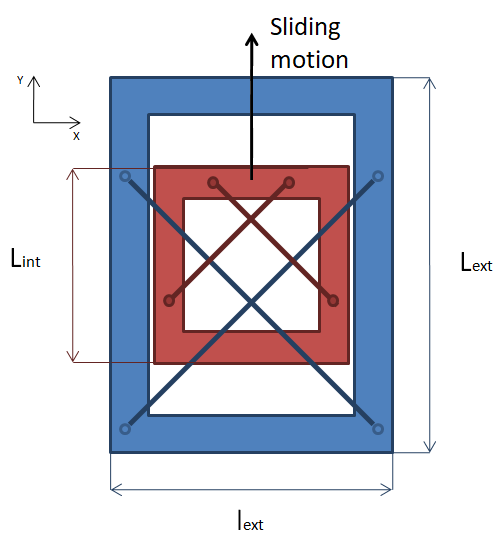
\includegraphics[width=0.4\textwidth]{archivos/baseline_device.png}
	\caption{Diagram of the baseline device}
	\label{device_baseline}
\end{figure}

The device had to accomplish two main objectives: 

\begin{itemize}
	\item to help prevent the influence of the boundary contitions, the minimum size of the stretched central square should have approximately a $6 \; \textrm{mm}$ long side; 
	\item and the size of the central square had to be small enough to hold a $2 \; \mu \textrm{L}$ spherical droplet when the device was shrunk. 
\end{itemize}

Since, at 40x magnification, we will examine $435 \; \mu \textrm{m}$ side squares, the maximum size intends to minimize the effects of the boundary conditions. The Stokes' paradox establishes that perturbations can be quite long ranged, but by looking at the center of the film we expect to be similar enough to the periodic boundary conditions considered in the simulations.

However, the second of this requirements was harder to foresee, and, knowing that the threads were flexible, somehow less important. This led us to the following measures:

\begin{equation}
	L_{ext} = 40 \; \textrm{mm}; \quad l_{ext} = 28 \; \textrm{mm}; \quad L_{int} = 20 \; \textrm{mm}; \quad t = 3.8 \; \textrm{mm}
\end{equation}

where $t$ represents the thickness of both frames.

For the threads we used a $50 \; \mu \textrm{m}$ diameter fishing line (see Fig. \ref{fishing_line}) that we glued to the frames . The frames were laser-cut from a $6 \; \textrm{mm}$ thick sheet.

\begin{figure}[H]
	\centering
	\includegraphics[width=0.3\textwidth]{archivos/fishing_line.jpg}
	\caption{Asso® micron 3 fishing line (D $50 \; \mu \textrm{m}$)}
	\label{fishing_line}
\end{figure}

To hold both frames at the same level, a thinner plastic sheet was glued to the bottom of the outer one.

The relative motion is achieved through the use of a $3 \; \textrm{mm}$ diameter screw. The external frame is drilled and threaded, whereas the internal one is only drilled. Finally, to prevent the screw from sliding back and forth relatively to the inner frame, we place two blocks on both sides of the drill hole.   

\begin{figure}[H]
	\centering
	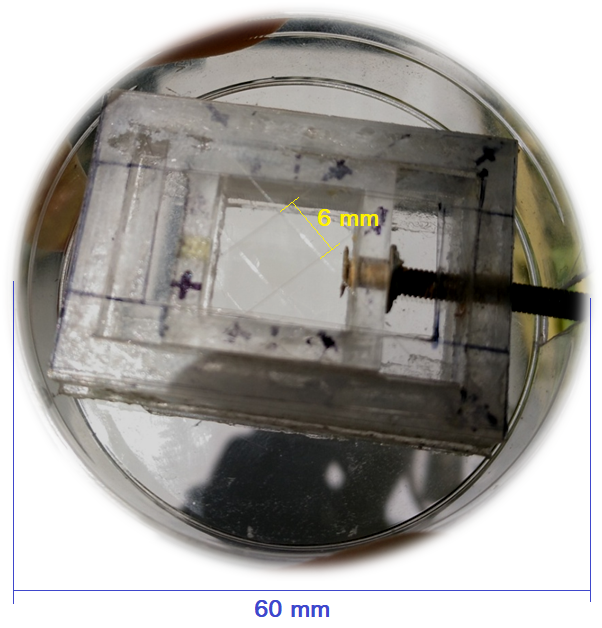
\includegraphics[width=0.4\textwidth]{archivos/device.png}
	\caption{Picture of the device}
	\label{device}
\end{figure}

Previous experiences, such as those of Guasto et al.~\cite{Guasto}, revealed that, at about $25^\textrm{o}\textrm{C}$, the evaporation was too intense for the film to hold long enough to obtain a sufficient number of images at the sought-after thickness. Their solution (and ours) to this problem consisted in enclosing the device in a small box. For this purpose we chose a petri dish (Fig. \ref{petri_dish}). We also placed a humid cotton inside the chamber to increase the saturation levels of the air within it.

\begin{figure}[H]
	\centering
	\includegraphics[width=0.4\textwidth]{archivos/petri_dish.jpg}
	\caption{Corning® tissue-culture treated culture dishes (mfr. no. 430196: D × H $60 \; \textrm{mm}$ × $15 \; \textrm{mm}$)}
	\label{petri_dish}
\end{figure}

The reduced microscope working distance obliges to place the film very close to one of the dish walls. So close that the initial droplet would touch it, precluding the possibility of closing the box before setting up the film.

\section{Microscopy}
\label{mm_microscope}

A Nikon® Eclipse Ti-U inverted microscope with a Nikon® MRP46402 objective (LWD 40x/0.55 Ph1 ADL ∞/1.2 WD 2.1) objective was used in this research together with a Photron® FASTCAM SA3 high speed camera.

This camera provides a 1024 x 1024 pixel resolution at frame rates well above the one we have used (i.e. $50  \; \textrm{fps}$). Under this format we can record up to 2726 images, that is to say $54.52 \; \textrm{s}$.

To prevent phototaxis, the illumination power must be reduced as much as possible. Moreover, the use of a red filter (Newport® FSQ-RG610 Colored Glass Longpass Filter: 50.8 x 50.8 $\textrm{mm}$, $610 \; \textrm{nm}$ cut-on optical filter) cuts the short wavelengths from the spectrum, to which \textit{Chlamydomonas reinhardtii} is most sensitive.

This also helps to prevent heating, and thus, thermotaxis, evaporation and air thermal convection within the petri dish.

\section{Thickness measurement}
\label{mm_thickness}

In order to estimate the volume of the droplet needed to obtain a $15  \; \mu \textrm{m}$ thick layer, we start by considering a uniform thickness (i.e. a $6 \; \textrm{mm} \times 6  \; \textrm{mm} \times 15 \; \mu \textrm{m}$ square cuboid). This leads to a volume of $0.5 \; \mu \textrm{L}$.

On the one hand, such a low volume is subject to a great level of uncertainty, on the other hand, we positively know that thickness is not uniform. This is why we finally opted to deposit a $ 2 \; \mu \textrm{L} $ droplet. The droplet was then let to evaporate until the desired thickness was reached. 

To measure the thickness, we use the microscope's fine focus knob. To do so we need to know the equivalent in $\mu \textrm{m}$ to a knob's turn. 

Two lines were drawn at the top and bottom of a $150 \; \mu \textrm{m}$ thick glass lamella and $112$ graduations of the knob were measured between those marks with a 60x magnification. 

The next figure shows the geometry of the refraction phenomenon:

\begin{figure}[H]
	\centering
	\includegraphics[width=0.7\textwidth]{archivos/Refraction.PNG}
	\caption{Schematics of refraction parameters}
	\label{refraction}
\end{figure}

We measured $L_a$ with the microscope, we knew the value of $L_i$ for the glass (or $L_g$), and we wanted to calculate $L_i$ for the water (or $L_w$). know the refraction indexes of both glass and water ($n_g = 1.45$,  $n_g = 1.33$) and with a simple geometric relationship (see Fig. \ref{refraction}):

\begin{equation}
\left.
\begin{aligned}
& \frac{h}{L_a} = \tan \theta_a \\
& \frac{h}{L_i} = \tan \theta_i
\end{aligned}
\right\}
\frac{L_a}{L_i} = \frac{\tan \theta_i}{\tan \theta_a} \simeq \frac{\sin \theta_i}{\sin \theta_a}
\end{equation}

And using Snell's law:

\begin{equation}
\left.
\begin{aligned}
& \frac{L_a}{L_i} \simeq \frac{\sin \theta_i}{\sin \theta_a} \\
& \frac{n_a}{n_i} = \frac{\sin \theta_i}{\sin \theta_a}
\end{aligned}
\right\}
\frac{L_a}{L_i} \simeq \frac{n_a}{n_i} 
\end{equation}

Which applied to both materials (glass and water):

\begin{equation}
\left.
\begin{aligned}
& \frac{L_a}{L_w} \simeq \frac{n_a}{n_w} \\
& \frac{L_a}{L_g} \simeq \frac{n_a}{n_g} 
\end{aligned}
\right\}
L_w \simeq L_g\frac{n_w}{n_g} 
\end{equation}

In conclusion, in our microscope, for a 60x magnification, $112$ graduations are equivalent to $138 \; \mu \textrm{m}$ in water.

\section{Cell culture}
\label{mm_culture}

For our purposes we have chosen an axenic broth culture of wild-type \textit{Chlamydomonas reinhardtii}, incubated at $21^\textrm{o} \textrm{C}$ under a 12 h bright/dark light cycle to optimize motility and cell size uniformity.

Other possibilities have been considered, such as a 14 hour light/10 hour dark cycle (recommended by ATCC\footnote{The American Type Culture Collection is a nonprofit organization that collects, stores, and distributes standard reference microorganisms, cell lines... for research purposes.} protocols). However, we wanted our results to be comparable to Kurtuldu's~\cite{Kurtuldu2011} and, as explained by Bruce~\cite{Bruce}, the circadian clock has a strong influence on reproduction and phototaxis. It has, as well effects on chemotaxis (see Byrne et al.~\cite{Byrne}).

The selected maintenance medium is Tris-acetate-phosphate (Gibco™ TAP Growth Media, optimized for Chlamydomonas culture: ref. A13798-01). 

Subcultures are performed regularly under the same conditions: every 7 days, we take $1 \textrm{mL}$ of the previous broth and add it to $24 \textrm{mL}$ of TAP, for a total volume of $25 \textrm{mL}$.

Higher concentrations of algae are achieved through centrifugation and resuspension\footnote{At least one hour is needed for resuspension and for the algae to resume their normal activity.} of the solution.

\section{Tracers}
\label{mm_tracers}

Following the procedures of both Kurtuldu et al.~\cite{Kurtuldu2011} and Guasto et al.~\cite{Guasto}, a part of the cell culture is mixed with $1 \; \mu \textrm{m}$ diameter fluorescent red polystyrene microspheres (ThermoFisher Scientific, ref.: R0100). 

We call this microspheres \textit{tracers} because they are supposed to follow (trace) the surrounding flow almost perfectly. For this to happen, they need to accomplish a certain condition. To understand what this condition might be, let us introduce the Stokes number:

\begin{equation}
St = \frac{t_p}{t_c}
\end{equation}

where $t_p$ is the relaxation time of the particle, and $t_c$ is a characteristic time of the flow. The latter is not univocally defined, but one of the usual choices is a convective time determined by the ratio of: $l_c$, which is the characteristic length of the obstacle (typically its diameter), and $u_c$, which is the fluid velocity away from the obstacle.

It follows that, for $St << 1$, particles follow the surrounding fluid closely, without altering it (they are tracers). After Tropea et al.~\cite{Tropea}, if  $St < 0.1$, tracing accuracy errors are below 1\%.

Let us then approximate the Stokes number of the microspheres to be aware of the error order. In the case of Stokes flow, which is ours, the particle drag coefficient is inversely proportional to the Reynolds number, and the expression of the Stokes number becomes:

\begin{equation}
	St = \frac{\rho_p d_p^2 u_0}{18 \mu_g l_c} \simeq 2.63 \cdot 10^{-4}
\end{equation}

as $\rho_p = 1.05 \; \textrm{g/cm}^\textrm{3}$, $d_p = l_c = 1 \; \mu \textrm{m}$, and we consider the worst-case scenarios regarding the temperature: $\mu_g(30^\textrm{o} \textrm{C}) = 7.98 \cdot 10^{-4} \; \textrm{kg/(m} \cdot \textrm{s)}$; and the speed, estimating that the tip-of-flagella\footnote{The length of the flagella is $l_f \simeq 10 \; \mu \textrm m $} velocity in a semicircular-like motion at $ f \simeq 60 \; \textrm{Hz}$ is, at most, of $ 2 \pi l_f f = 3600 \; \mu \textrm{m/s}$. This obviously constitutes an over-estimation of the Stokes number, whose value is still under 0.1, allowing us to state that the microspheres behave as tracers with high precision.

\section{Surfactants}
\label{mm_surfactants}

Two different types of surfactants have been used (separately) over this research: Sodium dodecyl sulfate\footnote{Cell membranes are sensible to this type of surfactant, so it can only be used in experiments without algae} (Roche®: SDS 11667289001 - CAS Number 151-21-3) and Polysorbate 20 (Sigma Aldrich: Tween® 20 P9416 - CAS Number 9005-64-5, MDL number MFCD00165986).
 
\begin{figure}[H]
	\centering
	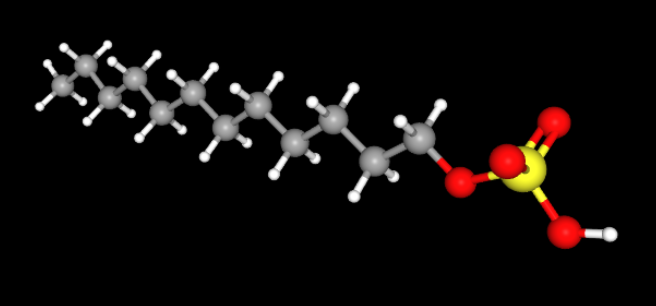
\includegraphics[width=0.7\textwidth]{archivos/SDS.PNG}
	\caption{Sodium dodecyl sulfate (SDS) molecule~\cite{SDS} (white=H, grey=C, red=O, yellow=S; sodium cation, $Na+$, not represented)}
	\label{refraction}
\end{figure}

Sodium dodecyl sulfate~\cite{SDS}, also known as Sodium Lauryl Sulfate (SLS) is an anionic surfactant naturally derived from coconut and/or palm kernel oil. SDS also has some microbicidal activity. Its molecular formula is $C_{12}H_{25}O_4S.Na$ and its molecular Weight, $288.38 \; \textrm{g/mol}$.

\begin{figure}[H]
	\centering
	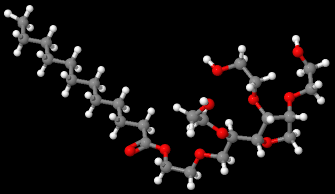
\includegraphics[width=0.7\textwidth]{archivos/Tween20.PNG}
	\caption{Simplified (missing PEG units) Polysorbate 20 (Tween® 20) molecule (white=H, grey=C, red=O)~\cite{Tween}(modified image)}
	\label{tween}
\end{figure}

Polysorbate 20 is a synthetic nonionic surfactant. The number 20 corresponds to the 20 repeat units of polyethylene glycol (PEG) in the polar head of the molecule. These units are distributed across 4 different chains, so in fact Polysorbate 20 consists of a range of chemical species.

Trace amounts of this substances lower the surface tension, helping the setup and improving the durability of the film. In the beginning we used SDS in low concentrations (always lower than its CMC, $8.2 \; \textrm{mM}$ at $25^\textrm{o} \textrm{C}$) in some films. Later, based on the paper of Kurtuldu et al.~\cite{Kurtuldu2011}, we used Tween 20, $0.03\%$ v~∕~v in some of our experiments.

\section{Staining}
\label{mm_staining}

In some experiments, if the initial thickness of the film was too high, and therefore, the evaporation time, very long, the algae would eventually stop moving before reaching the desired thickness, hampering the production of meaningful images/data.

This lack of motion can be due to either the death of the cells or the loss of their flagella. To know if it is one or the other, we decided to conduct a LIVE/DEAD Cell test. 

The test kit we will be using consists of calcein acetoxymethyl (\textit{calcein AM}) and ethidium homodimer-1 (\textit{EthD-1}). The former is a non-fluorescent compound that can be transported through the cellular membrane. Once inside the cell, the intracellular esterase activity removes the acetomethoxy group, so the molecule can no longer exit the cell and it exhibits a strong green fluorescence. The latter is a membrane-impermeable, high-affinity nucleic acid red stain that is weakly fluorescent until bound to DNA. When cells die, the plasma membranes break down, letting EthD-1 enter.

Noise levels out of the cells are weak since both dyes are almost non-fluorescent before interaction with the cells.

In conclusion, the test should show live cells stained with Calcein-AM (green) and dead cells with EthD-1 (red). Nonetheless, it should be noted that the test kit we will use is designed for mammalian cells (ThermoFisher Scientific LIVE/DEAD™ Viability/Cytotoxicity Kit, for mammalian cells: ref. L3224). \textit{Chlamydomonas reinhardtii} presents a cell wall which, although cellulose-deficient~\cite{Imam}, may interfere with the staining. Nonetheless, previous successful experiences with bacteria, that are also wrapped in a cell wall, encourage the realization of the experiment. 

The original protocol for mammalian cells is the following one:

\begin{itemize}
	\item Prepare $2 \; \mu \textrm{L}$ calcein and $4 \; \mu \textrm{L}$ Eth-D in 1mL EC media.
	\item Wash system with PBS
	\item Inject live/dead in the system, place in incubator for 30 minutes.
	\item Remove live/dead and wash with PBS. Wait for 5 minutes.
	\item Refresh PBS. Wait for 5 minutes.
	\item Image live/dead.
\end{itemize}

It is intended to discern which cells are dead or alive at the time when they are stained. We, on the contrary, would like to acquire a more \textit{dynamic} information: if cells that were alive at the beginning of the experiment are dying over it. This is why our protocol becomes:

\begin{itemize}
	\item Centrifugate ($600 \; \textrm{g}$, $6 \; \textrm{minutes}$) and replace the algae medium (TAP) 3 times.
	\item Get 0.2mL of the desired concentration by centrifugation. 
	\item Prepare $2 \; \mu \textrm{L}$ calcein and $4 \; \mu \textrm{L}$ Eth-D in $0.8 \; \textrm{mL}$ TAP media.
	\item Wash system with ethanol.
	\item Wash system with distilled water.
	\item Inject live/dead in the system.
	\item Image live/dead.
\end{itemize}

%https://www.thermofisher.com/order/catalog/product/L3224

	\chapter{Results and analysis}
\label{results_analysis}

Given that this research is to be continued in the following months, this report must be considered as an intermediate stage. Still, some coherent results have been found and, more importantly some of the side problems have been explained and mitigated within our means.

For the sake of clarity, this section is going to be presented in a mostly chronological way (with a final summary of the results). This will allow us to present the problems, solutions and results in a logical way.

Luckily, once the device was built and with an almost constant supply of cells (contamination issues aside), experiments are quite fast and we have been able to run close to $100$ of them.

We want to quickly recall the aim of our experiments and the protocol followed in each of them. Regarding the aim, we intend to study the influence of Chlamydomonas reinhardtii on the diffusion of micrometric tracers in a 2-dimensional environment. Concerning the protocol, we first prepare an aliquot of the algae in their medium (higher levels of concentration are achieved by centrifugation). Then, we add the tracers and, if required, the surfactant. Some wet cotton is to be put in the box if we want to prevent evaporation. We \textit{close} the device (approaching its threads) and, with the help of a pipette, we put a droplet of the desired volume between the threads, touching them. With the help of the device, we pull the threads $6 \; \textrm{mm}$ away, so as to have a thin square film, and we cover the box. Finally we turn the box upside down and we put it under the microscope, where we will wait for it to reach the expected thickness. Then we acquire images for approximately 1 minute. One of the resulting images can be seen on Fig. \ref{frame_e3}

\begin{figure}[H]
	\centering
	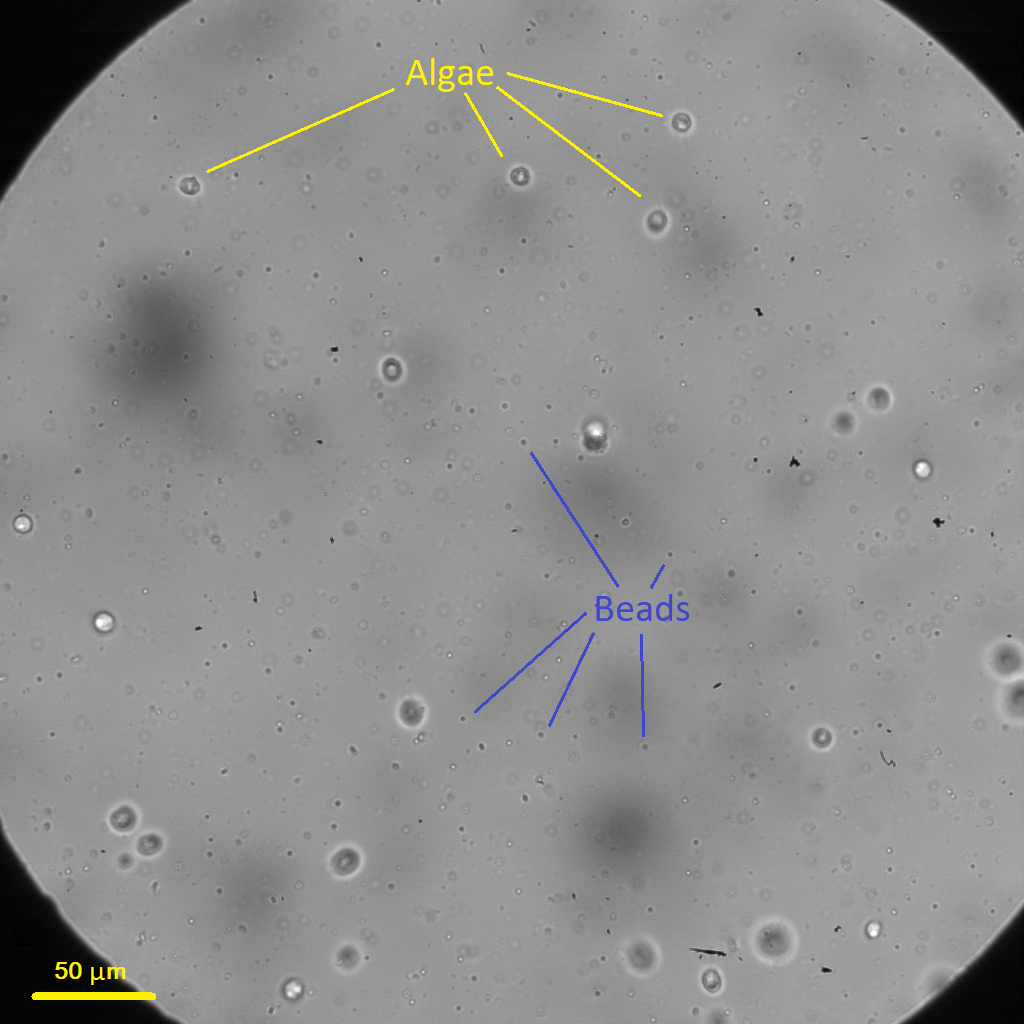
\includegraphics[width=0.65\textwidth]{archivos/e3_randomframe.png}
	\caption{Example of the frames obtained throughout the experiments}
	\label{frame_e3}
\end{figure}

As it has been explained in section ¿¿¿5.1???, diffusion can be quantified by measuring the MSD of tracers as a function of the elapsed time. This is why, in our images, we will look for the displacements, $\Delta x$ and $\Delta y$, of the tracers along the axes of the selected reference frame (usually the laboratory reference frame) for different elapsed times, $\Delta t$.

Among our experiments, most were devoted to assess the diffusion of tracers in the presence of \textit{Chlamydomonas reinhardtii}. However, a non-negligible amount of them had other purposes such as evaluating the effects of evaporation, surfactants, tilt,... This already reduces the number of available data, but much more importantly, we have not been able of exploiting most of the images satisfactorily.

The first and main reason for this is the presence of \textit{background flows}. Afterwards, as a consequence of the implemented solutions further problems arose such as the premature death of algae or the presence of quiescent beads on the surfaces of our film.

\section{Background flow}

Fig. \label{backg_flow} shows a projection of the darkest points of a series of frames (over $5.5$ seconds). This allows us to see the particle and algae paths.
The particle paths in Fig. \label{backg_flow} show a \textit{mean} behavior that is neither Brownian nor related to the algae kicks.

\begin{figure}[H]
	\centering
	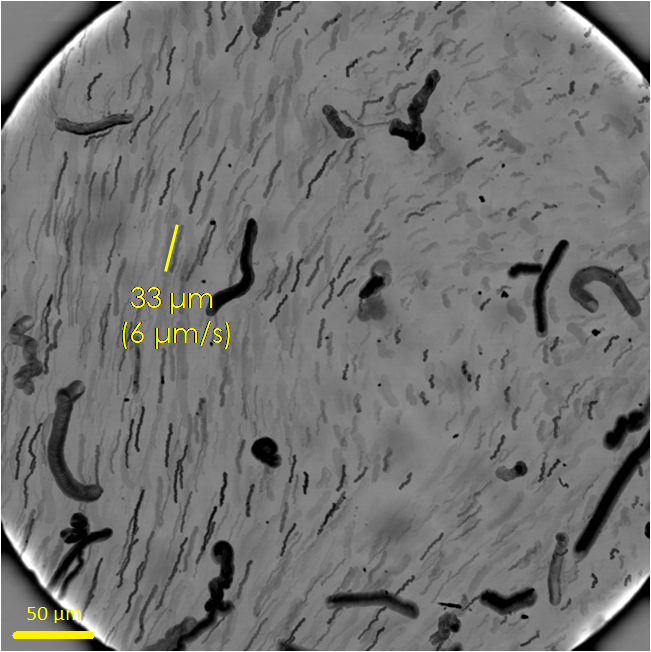
\includegraphics[width=0.65\textwidth]{archivos/backg_flow.png}
	\caption{The common trend of the streamlines (over 5.5 seconds) in the left part of the image suggests the presence of a background flow. It reflects a velocity magnitude of the order of $6 \mu m / s$}
	\label{backg_flow}
\end{figure}

We call \textit{background flow} to these currents, whose origin is unrelated to the presence of the algae.

If the background flow were uniform, we could think of simply removing its mean numerically, but it is not the case as one can see from the figure above. 

This led us to two possibilities: either developing more complex data processing algorithms or trying to improve our experiment setup. 

\subsection{Experimental removal}

\subsubsection{Possible causes of the background flow}

To remove this flow experimentally, we first need a better understanding of what is going on. Several hypothesis were proposed:

\begin{itemize}
	\item Evaporation
	\item Convection
	\item Marangoni stresses
	\item Tilt of the device
\end{itemize}

\subsubsection{Expert advice}

Since our setup had already been used by several authors in their articles, one of our first steps was to contact one of them: Dr. Jeffrey S. Guasto. Here are some of the pieces of advice he gave us in answer to our questions and our reactions to them:

\begin{itemize}
	\item \textit{We did not have a major problem with background flows. But depending on what you are looking at and length scale of the background flow, you could consider subtracting the mean from your flow of interest.}
\end{itemize}

We will consider this and other options for numerically removing the background flow in the next section.

\begin{itemize}
	\item \textit{Thin films are fundamentally quite temperamental: related to Stokes' paradox where perturbations can be quite long ranged, and actually the over side length of the film can play an important role in its behavior (not just the thickness).}
\end{itemize}

It would probably take another research project to properly analyze the effects of our boundary conditions on our problem. This is the reason why we opted for a more empiric approach, choosing the size of our layer based on previous works, such as Guasto's himself. Our film is a $6mm$ side square, whereas his is $5mm$, so this should not be a problem.

\begin{itemize}
	\item \textit{Regarding our chamber and setup: We used a similar method of humidifying the chamber to help prevent evaporation. We also blocked as many openings from the top of the sample holder and the bottom side (i.e. opening in the stage where the objective protrudes). We tried to make this enclosure as small as possible - ours measured approximately 5cm x 5cm x 5mm. The small size helps to maintain humidity and also to prevent air circulation inside of the chamber (e.g. natural convection due to slight heating). For the light source, you should aim to minimize the illumination power and of course if working with Chlamy, short wavelengths should be cut from the spectrum to avoid inadvertent phototaxis - this also helps to prevent heating though.}
\end{itemize}

The humidifying method we use consists in putting a wet cotton at the bottom of the box. 

By using a Petri dish, we managed to place the film close enough to the top cover so to have it within the \textcolor{red}{¿¿¿ focal range ???}, avoiding the need for an extra opening. 

The Petri dish inner diameter is $\phi = 5 \; \textrm{cm}$ and its height is $h = 1.3 \; \textrm{cm}$. This means our volume is $\sim 2$ times theirs, but further diminishing the height of the box does not seem to improve our situation.

Concerning the light source, we work with the minimum intensity of light allowing to obtain clear images of the algae and the tracers. We use as well a red filter to avoid phototaxis. Indeed, longer wavelengths are less energetic and the heating should be less intense.

Regarding other possible sources of taxis: given the low thickness of the films we will be working with, the effects of aerotaxis and gravitaxis should be negligible. A correct mixing of the suspension should prevent chemotaxis as well. Thermotaxis could constitute a problem, but the use of red light mitigates it. The red filter should also reduce the thermal- and evaporation-induced flows, and thus rheotaxis. To avoid barotaxis and thigmotaxis, the observed area must be far enough from the borders of the domain. 

\begin{itemize}
	\item \textit{Regarding the fluid (...), we found that the cells were very sensitive to the surfactant concentration, and thus we minimized the concentration to ensure their motility in spite of any benefits to the film mechanics. I think that we found a concentration right around the CMC \footnote{Critical micelle concentration defined as the concentration of surfactants above which micelles are spontaneously formed~\cite{Sheng2011}} for Tween 20 worked best to maintain both the film and the cell motility. To properly control surfactant concentration - if using commercially available tracer particles - it is also critical to wash the tracers and remove the harsh surfactants in which they are packed (again for the sake of the cells).}
\end{itemize}

For the first tests without algae but with beads, we used SDS to help maintain the film, but shortly after we noticed that there was no need for it, since our layers were relatively easily formed and remained there long enough.

Based on Guasto's advice, we started washing the tracers, and even the algae, right before the experiments, to make sure the concentration of surfactants was as low as possible. The problem is that traces are always present and even the slightest concentrations can have important effects as we will see later.

So, at a certain point, we also decided to try and use Tween 20 in some of our experiments to reproduce Guasto's experiment as accurately as possible, since he did not find such problems. This does not seem to work though.

\begin{itemize}
	\item \textit{Regarding the (...) film: The films are relatively short lived and are constant thinning (there is no way to prevent this - some experiments increase the fluid viscosity to slow thinning, but this has obvious issues with swimmers). Our approach was to pull the film to a fixed size ($ \sim 5 \; \textrm{mm}$ square if I recall) and wait for it to thin to our desired thickness ($ \sim 10-15 \; \mu \textrm{m} $). Once it reached the required thickness, we would acquire data for about $1-3 \; \textrm{minutes}$ while the film remained in this thickness range. The film is also not of uniform thickness and all of our data was acquired in the central $ \sim 1 \; \textrm{mm}^2 $.}
\end{itemize}

It is true that at the beginning, before using the wet cotton, our films were shorter lived, but after that this was not a problem anymore and our layers would endure up to several hours. This allows us to neglect the thickness variation over our experiments (each video lasts around $50-55 \; \textrm{seconds}$.), and suggests that evaporation should not be responsible for the background flows.

Acquiring the data from the central $ \sim 1 \; \textrm{mm}^2 $ is not always easy. Firstly, because it is hard to measure, secondly, because we try to find regions with the lowest number of dead algae and with representative concentrations. Nonetheless, we stay as far away as possible from the edges to prevent boundary effects and work with nearly constant thickness.

To be more precise, if we resume the equations developed in section ¿¿¿3.1.5???, for the values $R = 3 \; \textrm{mm}$, $\rho = 25 \; \mu \textrm{m}$ and $\theta = 70^\textrm{o}$, $h_0 = t/2 = 7.5 \; \mu \textrm{m}$, which are similar to the dimensions of our film, we obtain $B \simeq 6.90 \cdot 10^{-4}$ and a volume of $ \simeq 0.45 \; \mu \textrm{L}$. The shape of the film is shown in the next figures:

\begin{figure}[H]
	\centering
	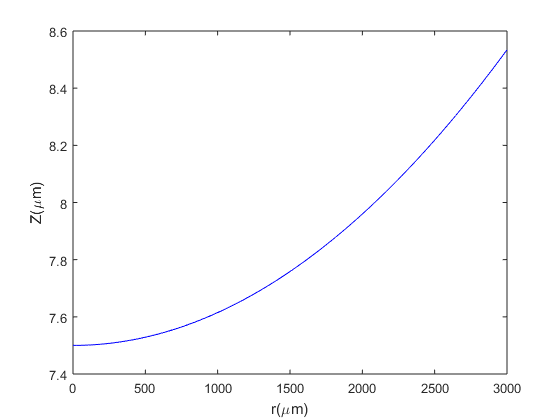
\includegraphics[width=0.6\textwidth]{archivos/CircFilmFunction.png}
	\caption{Half thickness of the film as a function of the radial position.}
	\label{CircFilmFunction}
\end{figure}

\begin{figure}[H]
	\centering
	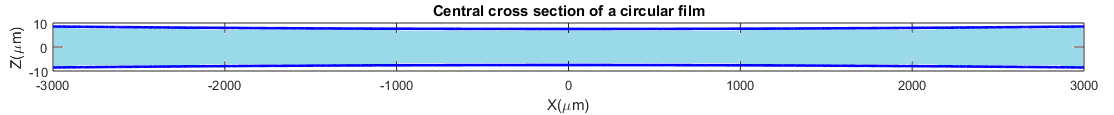
\includegraphics[width=\textwidth]{archivos/CircFilmSection.png}
	\caption{Diagram of a the liquid film next to the thread.}
	\label{CircFilmSection}
\end{figure}

Far enough from the boundary conditions we can expect a similar shape for a square shaped film, so indeed we can consider that it is mostly flat.

\subsubsection{Other possible causes}

Besides these pieces of advice, other possibilities were contemplated.

For instance, we also considered Marangoni stresses that, acting on the surface, are very effective in generating currents in the bulk. We are not sure whether or not they play a major role, but, if that is the case, very little can be done to mitigate them, since, as we have already mentioned, even the smallest concentrations can have important effects.

This leaves us with the last option: the tilt of the device which is completely unavoidable to a certain extent.

To find out the magnitude of the tilt angle needed to reach the mean velocity of our tracers ($\sim 6 \; \mu \textrm{m/s}$), we may now bring back the equations in section ¿¿¿4.5??? and calculate the orders of magnitude of the different terms. 

Before doing so, we first need to establish the hypothesis to assess some values:

\begin{itemize}
	\item Regarding the 2D viscosity, it should be measured experimentally, but we do not have the time to do so. Since we have a negligible surfactant concentration, we will estimate it as $\mu_{2D} \sim h \cdot \mu \sim 1.5\cdot 10^{-5} \cdot 1\cdot 10^{-3} \sim 1.5\cdot 10^{-8} \; \textrm{kg/s}$.
	\item Our characteristic velocities must accomplish $ v_{\mathrm{ac}} \sim v_c \sim 6 \; \mu \textrm{m/s}$ and $ v_{\mathrm{ac}} < v_c $.
	\item We know $x_{\mathrm{ac}} \sim x_c$, and in our problem $ x_c \sim z_c $ and $ x_{\mathrm{ac}} \sim z_{\mathrm{ac}} $ (both geometrically and because of the second Eq. \ref{air_velocity}), so, in conclusion, $ x_{\mathrm{ac}} \sim x_c \sim z_{\mathrm{ac}} \sim z_c \sim 3 \; \textrm{mm}$
	
\end{itemize}

So the terms in equation \ref{film_velocity}:

\begin{equation}
\left\{
\begin{aligned}
& \mu_{2D} \frac{d^{2} v(x)}{d x^{2}} \sim \frac{1.5\cdot 10^{-8} \cdot 6\cdot 10^{-6}}{(3\cdot 10^{-3})^2} \sim 1\cdot 10^{-8} \; \textrm{kg/(m} \cdot \textrm{s}^\textrm{2} \textrm{)}\\
& 2 \mu_{\mathrm{a}}\left|\frac{\partial v_{a}(x, z)}{\partial z}\right|_{z=0^{+}} \sim 2 \cdot 1.8\cdot 10^{-5} \frac{6\cdot 10^{-6}}{3\cdot 10^{-3}} \sim 7.2\cdot 10^{-8} \; \textrm{kg/(m} \cdot \textrm{s}^\textrm{2} \textrm{)}\\
& \rho h g \sin \alpha \sim 1\cdot 10^{3} \cdot 1.5\cdot 10^{-5} \cdot 1\cdot 10^{1} \cdot \sin \alpha \sim 1.5\cdot 10^{-1} \cdot \sin \alpha \; \textrm{kg/(m} \cdot \textrm{s}^\textrm{2} \textrm{)} 
\end{aligned}
\right.
\end{equation}


This means that the third term must as well be of the same order which leads to $\sin \alpha \sim  \alpha \sim 1\cdot 10^{-7} \; \textrm{rad} \sim (1\cdot 10^{-5})^\textrm{o}$.

This is equivalent to a slope of $10 \; \mu \textrm{m}$ every $\textrm{m}$, which is, of course unavoidable in our experiences.

\subsubsection{How to mitigate the existing background flow}

Sometimes, however, we do not appreciate this effects in all of the experiences: why would this be? Equation \ref{film_velocity} gives us a hint. It is clear that the most important source of currents, besides the tilt, is going to be the handling of the device (i.e. putting it under the microscope after settling the film). It is the surface viscosity, $\mu_{2D}$, which determines the level of dissipation\footnote{higher values of $\mu_{2D}$ should increase dissipation} so, if we start with a thicker layer, these currents should be dampened.

As Guasto does, we decided then to start from a higher thickness and wait for it to reach the expected value thanks to evaporation. This strongly diminished the levels of \textit{background flow}.

\subsubsection{Thickness measurement and evolution}

When it comes to measuring the thickness, we have several options. Given our concept of 2-dimensionality (we need to have a film whose thickness is approximately equal to the diameter of an alga), the first option is to wait until we have a single layer of algae: they do not swim under or over one another and they remain more or less in the same focal plane.

\begin{figure}[H]
	\centering
	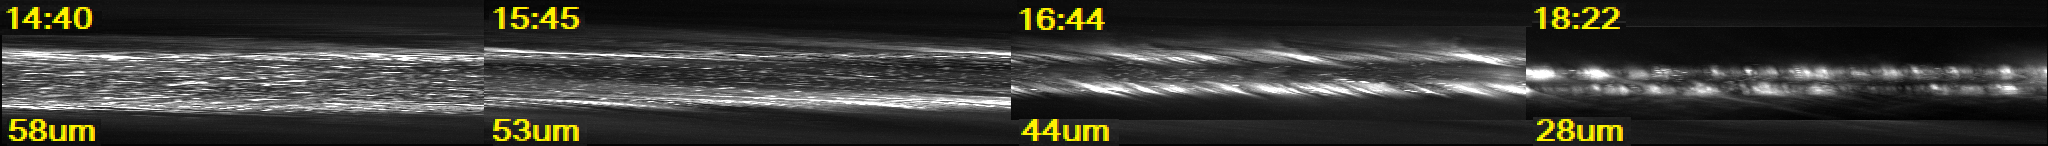
\includegraphics[width=\textwidth]{archivos/ThicknessEvolution.png}
	\caption{Evolution of the cross section of a film (time and thickness specified). Images obtained by fluorescence.}
	\label{thickness}
\end{figure}

The second option is to use the microscope to do a series of tomographies (with natural light or fluorescence), which would allow us to reconstruct the film in 3D (see Fig. \ref{thickness}). This technique is too slow, so, instead we used the focus knob to estimate the position of the bottom and the top of the layer (i.e. the position of the first and last tracers in focus)\footnote{The real thickness is not a direct output of this measurement. The procedure to obtain this value is explained in ¿¿¿ Materials and Methods ???}. In Fig. \ref{evap_rate} we can see the results of these measurements for an experiment where the box is closed with a wet cotton inside:

\begin{figure}[H]
	\centering
	\includegraphics[width=0.7\textwidth]{archivos/EvapRate.png}
	\caption{Cross section of a film over time.}
	\label{evap_rate}
\end{figure}

On the basis of this measurements, the calculated evaporation rate (slope of the curve) is about $ 0.61 \mu \textrm{m/min}$. \textcolor{red}{¿¿¿ COMMENT --> Negligible or not ???}

In addition to the temporal evolution of the film thickness, Fig. \ref{thickness} illustrates that, as expected, the fluorescent beads tend to accumulate at the surfaces. A trend that, logically, becomes more pronounced over time, since this diminishes the free surface energy. As we will see later, this can be a problem, but it makes it easier to measure the thickness.

\subsection{Numerical removal}

Background flows can be seen either in the microscope images and in the trajectories resulting of particle tracking. This algorithm outputs the particle and algae positions in every frame. Knowing the frame rate of the imaging, one can build the trajectory as a function of time. An example of tracers and algae trajectories can be seen in Fig. \ref{trajectories_e3}.

\begin{figure}[H]
	\centering
	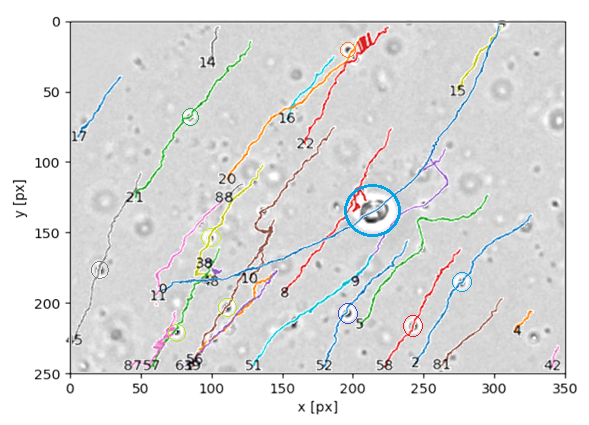
\includegraphics[width=0.8\textwidth]{archivos/trajectories_e3.png}
	\caption{Trajectories obtained by means of particle tracking superposed to one of its frames. An alga and some tracers are signaled by circles.}
	\label{trajectories_e3}
\end{figure}

The presence of a background flow, headed from the left-bottom corner to the right-top  is rather obvious on Fig. \ref{trajectories_e3}. 

Since disposing of background flows experimentally was not easy, we decided to explore the numerical removal in parallel.

\subsubsection{Initial approach: dismissed ideas}

Some initial ideas were put into practice and the dismissed. The main reason for this was that most of them were arbitrary in the sense that they depended on one or more subjective parameters (i.e. parameters that had to be chosen by the user). 

For instance, one of the first ideas was to split the tracers in two groups: those whose motion was affected by the presence of algae and those who were not. Once the classification done, the flow field provided by the non-affected group would be considered as the background flow and could be removed from the trajectories of the rest of the tracers.

Besides the inconvenience of having to choose a parameter whose value would determine if a bead was or not affected by the presence of algae\footnote{For this purpose we had chosen the distance to the closest alga.}, this method needed of a huge amount of tracers for the interpolation of the field to be successful. 

\subsubsection{Motion sources}

At this point, one might wonder where the difficulty lies when trying to remove this background flows. The beads motion is composed of three parts:

\begin{itemize}
	\item Brownian motion
	\item Motion induced by the algae 
	\item Motion induced by the background flow
\end{itemize}

Each of which is characterized by their own length and time scales. This makes it rather easy to isolate Brownian motion from the other two, because scales are very different, but when it comes to distinguish the algae contribution from the background flow, the separation is vaguer.

\subsubsection{Change of reference frame}

This is the reason why finally we decided to remove the background flow by working in a reference frame attached to the alga (see Fig. \ref{alga_RF}). The $X$ axis of this frame would be parallel to the alga's velocity vector at all times.

\begin{figure}[H]
	\centering
	\includegraphics[width=0.4\textwidth]{archivos/algaRF.png}
	\caption{Schematics of the alga reference frame ($\mathbf{v}_{alga}$ is the velocity of the alga in absence of external flows, and $\mathbf{v}_{bf}$ is the velocity induced by the background flow on the alga)}
	\label{alga_RF}
\end{figure}

Since every alga behaves in a different way, this idea had an obvious problem: controlling concentration. Nonetheless, in their paper, Kurtuldu et al.~\cite{Kurtuldu2011}, explain and demonstrate experimentally that, for low levels of concentration, where one can ignore the interactions between algae (i.e. in the dilute limit), considering the tracers within a circle (with variable radius) around each alga only is equivalent to modifying concentration.  

When we speak about concentration we refer to a 2D concentration, defined as:

\begin{equation}
\Phi = \frac{n \cdot A_{alga}}{S}
\label{concentration}
\end{equation}

where $n$ is the number of algae in the image, $A_{alga}$ cross section of the alga, and $S$ is the total surface of the image.

\begin{figure}[H]
	\centering
	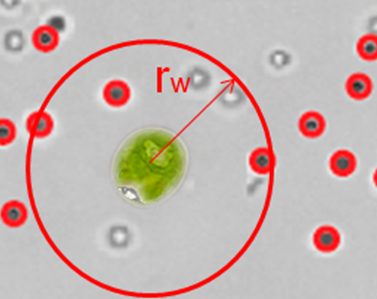
\includegraphics[width=0.4\textwidth]{archivos/concentration_circle.png}
	\caption{Specimen of \textit{Chlamydomonas reinhardtii} surrounded by tracers~\cite{chlamy_circ}. The radius of the surrounding circle determines the concentration of algae within it.}
	\label{concentration_circle}
\end{figure}

Applying this definition to the circle (see Fig. \ref{concentration_circle}) and supposing the area of an alga can be approximated by a circle whose radius is $r_{alga}$, we obtain:

\begin{equation}
\Phi = \frac{\pi r_{alga}^2}{\pi r_w^2} = \left(\frac{r_{alga}}{r_w}\right)^2
\label{conc_circle}
\end{equation}

After this small subsection, we have to focus again on the removal of the background flow by means of a change of the reference frame.

Although the Stokes number of the algae and the tracers is slightly different, we can consider that both are similarly affected by the background flow. Thus, in a mobile reference frame, background flow disappears.

Hereafter we present the pseudocode corresponding to this algorithm:

%--------------------------------------------------
\fbox{
	\begin{minipage}{15.4 cm}
		
		\vspace{0.2 cm}
		
		\textbf{Change of reference frame} 
		
		\vspace{0.2 cm}
		
		\hrule
		\vspace{0.4 cm}
		
		\textbf{Initialisation:} reading of the trajectories data (algae and tracers) and writing them on two dataframes belonging to two separate TrajectorySequence objects
		
		\vspace{0.2 cm}
		
		\textbf{Removal of the algae's Brownian motion and noise:}
		application of a \textit{derivative\_filter} to the algae trajectories
		
		\vspace{0.2 cm}
		
		\textbf{Cycle over different $\Delta t$:} repeat:
		
		\vspace{0.2 cm}
		
		\quad \textbf{Preparing parallelization:} splitting of the dataframe containing the tracer's 
		
		\quad trajectories
		
		\vspace{0.2 cm}
		
		\quad \textbf{Cycle over the existing algae:} repeat:
		
		\vspace{0.2 cm}
		
		\quad \quad \quad \textbf{Calculation of the alga direction:} we take the mean direction over $\Delta t$
		
		\vspace{0.2 cm}
		
		\quad \quad \quad \textbf{Parallel calculation of relative motion:} modulus and direction (and 
		
		\quad \quad \quad subsequent projection) of the tracers in the new frame of reference
		
		\vspace{0.2 cm}
		
		\quad \textbf{Definition of the circle around the alga} based on the desired concentration
		
		\vspace{0.2 cm}
		
		\quad \textbf{Discarding trajectories} out of the circle
		
		\vspace{0.2 cm}
		
		\quad \textbf{Saving the data} to a .csv file
		
		\vspace{0.2 cm}
		
		\textbf{Merging .csv files}
		
	\end{minipage}
}
%--------------------------------------------------

\subsubsection{First set of images: pushers}

After a few attempts we obtained a clear set of images (always presenting a background flow), with a sufficient concentration of tracers and algae. This set had the particularity that the algae would behave as pushers, as it can be seen on Fig. \ref{chlamy_pusher}. 

\begin{figure}[H]
	\centering
	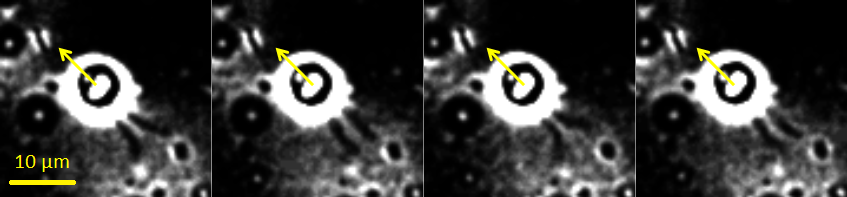
\includegraphics[width=0.8\textwidth]{archivos/chlamy_pusher.png}
	\caption{\textit{Chlamydomonas reinhardtii} behaving as a pusher (images every 0.02 seconds). The arrow indicates the direction of motion and the two flagella can be seen on the rear part of the alga.}
	\label{chlamy_pusher}
\end{figure}

This anomalous behaviour, explained in the \textcolor{red}{¿¿¿State of the art???} section, should not affect the shape of the distribution functions we are going to be looking for, but only their scales. We can, therefore, use this images to test our algorithm.

\subsubsection{Image processing}

The images have been processed to improve the performance of the particle tracking algorithm (see Fig. \ref{orbpe3}). The process consists in:

\begin{figure}[H]
	\centering
	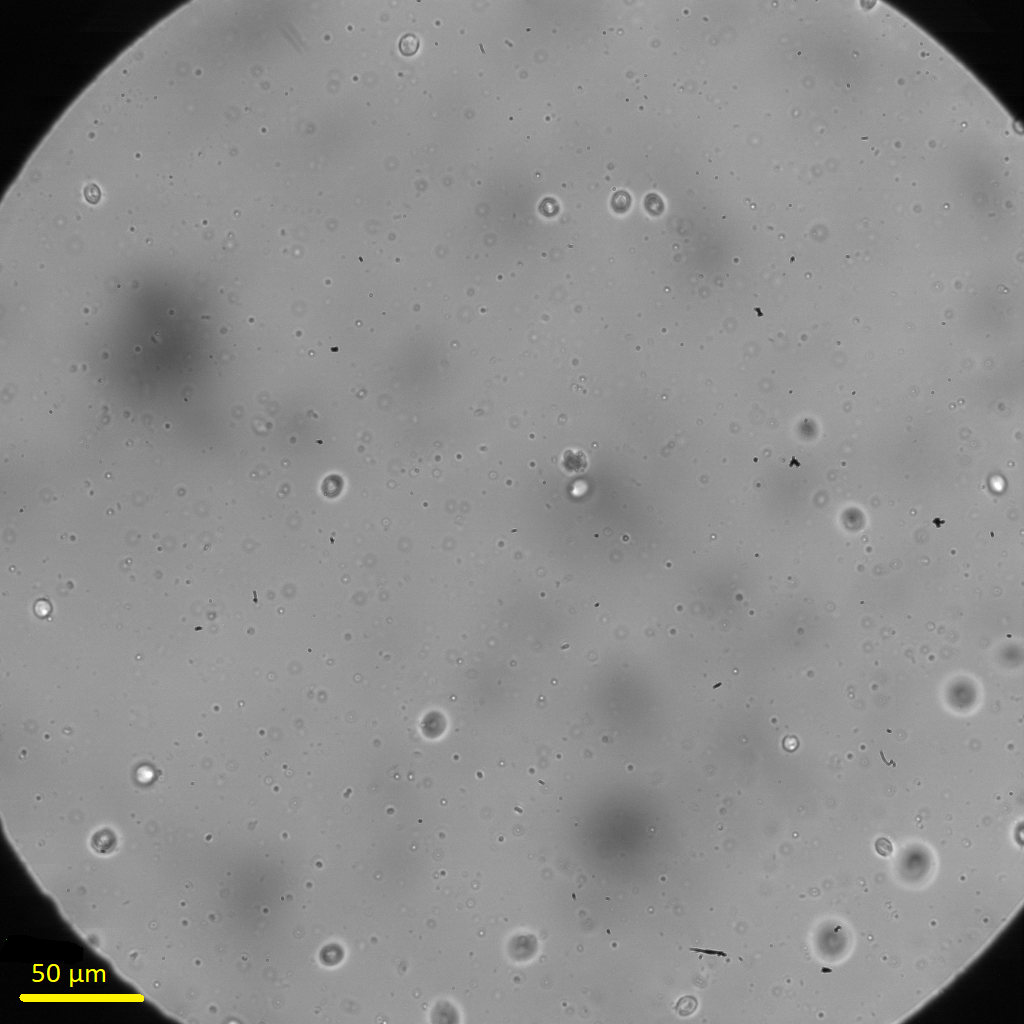
\includegraphics[width=0.4\textwidth]{archivos/frame_01_e3.png}
	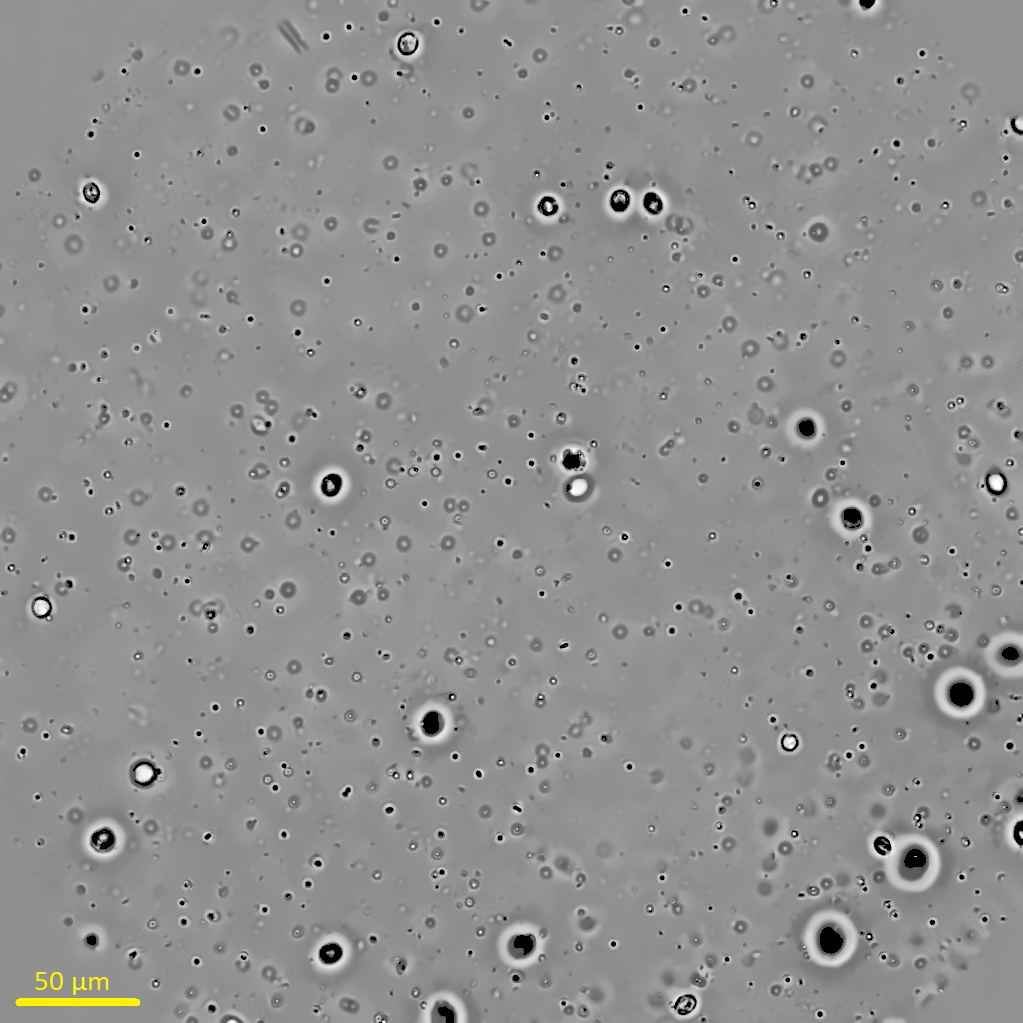
\includegraphics[width=0.4\textwidth]{archivos/frame_01_e3_bp.png}
	\caption{Original (left) and processed (right) frames.}
	\label{orbpe3}
\end{figure}

\begin{itemize}
	\item finding a mean image (over approximately 2700 frames), which is very similar to the background,
	\item removing this background of all the frames,
	\item applying a bandpass filter to highlight the structures, whose size is in the searched range,
	\item equalizing the set of images,
	\item improving contrast locally,
	\item denoising,
	\item and thresholding
\end{itemize}

\subsubsection{Application and results}

Fig. \ref{prob_dist_e3} shows the probability distributions of $\Delta x$ and $\Delta y$ (in the relative frame) for a fixed $\Delta t = 0.04 \; \textrm{s}$ and a concentration\footnote{The selected concentrations result of considering circles whose diameters are: \\ 
	$ \Phi \simeq 0.3\% \rightarrow r_w = 93.03 \; \mu \textrm{m} $ \\
	$ \Phi \simeq 0.7\% \rightarrow r_w = 60.90 \; \mu \textrm{m} $ \\
	$ \Phi \simeq 2.7\% \rightarrow r_w = 31.01 \; \mu \textrm{m} $} 
$\Phi = 0.674$ :

\begin{figure}[H]
	\centering
	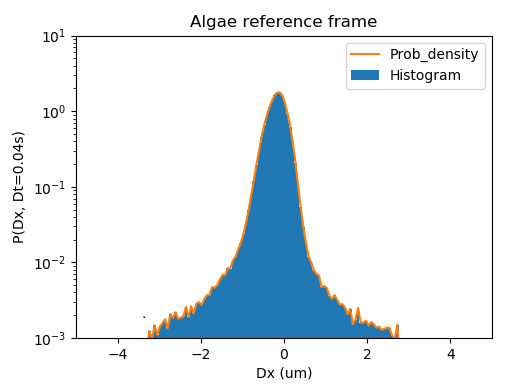
\includegraphics[width=0.42\textwidth]{archivos/pdf_x_e3.png}
	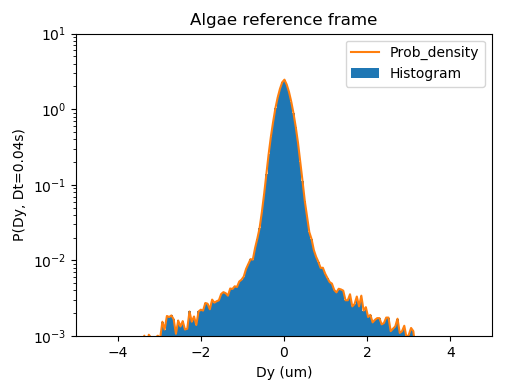
\includegraphics[width=0.4\textwidth]{archivos/pdf_y_e3.png}
	\caption{Histograms and probability distributions of the displacement $\Delta x$, (along the algae direction vector) and $\Delta y$ (perpendicular to it) in the turning reference frames attached to the algae, for a fixed $\Delta t = 0.04 \; \textrm{s}$ and $\Phi = 0.674$.}
	\label{prob_dist_e3}
\end{figure}

If background flow and algae motion were uniform, we would expect to find a $\Delta x$ distribution centered on $-\| \mathbf{v}_{alga} + \mathbf{v}_{bf} \|$. In fact, reality is more complex than that and both the background flow and the velocities of the algae are subject to distribution. Even if the velocity modulus were always the same in the straight parts of the paths, the behavior of the different individuals is usually defined as a mix between \textit{run-and-tumble} and directed phototaxis~\cite{Polin}. The term \textit{run-and-tumble} describes a motion where straight paths are followed by abrupt changes in the direction of the trajectory. For this changes to occur, the modulus of the velocity goes to zero (or close to it), which partially explains the dispersion of the velocity values.

To confirm this hypothesis, one can have a look at the distributions for longer $\Delta t$ (see Fig. \ref{prob_dist_e3_longer}), where the dispersion of the algae displacements must be remarkably higher.
 
\begin{figure}[H]
	\centering
	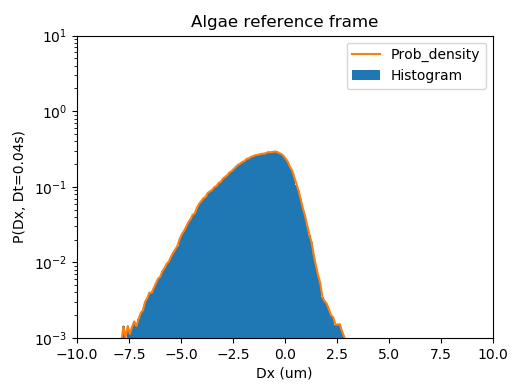
\includegraphics[width=0.42\textwidth]{archivos/pdf_x_e3_longer.png}
	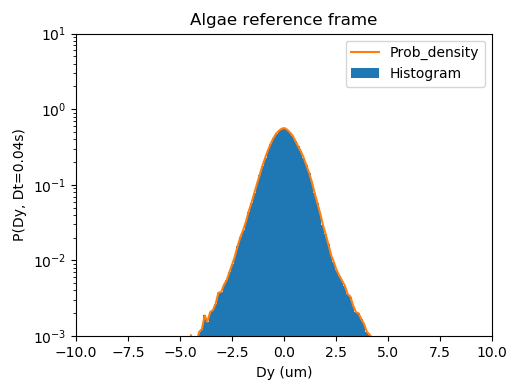
\includegraphics[width=0.4\textwidth]{archivos/pdf_y_e3_longer.png}
	\caption{Histograms and probability distributions of the displacement $\Delta x$, (along the algae direction vector) and $\Delta y$ (perpendicular to it) in the turning reference frames attached to the algae, for a fixed $\Delta t = 0.34 \; \textrm{s}$ and $\Phi = 0.674$.}
	\label{prob_dist_e3_longer}
\end{figure}

Since we ignore the distribution function of the algae velocities, let us focus on $\Delta y$. Kurtuldu et al.~\cite{Kurtuldu2011} suggest that, in the dilute limit, the probability distribution function is Gaussian, with Power Law tails. The Gaussian core corresponds to the pure Brownian motion, whereas the tails correspond to high amplitude, low probability events, that is to say, the algae kicks. 

We can fit an \textit{ad hoc} distribution to our data. The chosen distribution considers positive values only (we take the absolute value of the data) and consists of a Gaussian core, Power Law tails and a transition region. Even ignoring what the real transition law might look like, we can obtain a reasonable fitting just by imposing:

\begin{equation}
\int_{-\infty}^{\infty} f_x(x) dx = \int_{0}^{\infty} f_x(x) dx = 1
\label{probarea}
\end{equation}

where $f_x(x)$ is the probability density function, that we defined as: 

\begin{equation}
f_x(x) = \left\{
\begin{aligned}
& C_g \frac{2}{\sqrt{2 \pi \sigma^2}} e^{\frac{-x^2}{2 \sigma^2}} & \quad \textbf{if} \quad x \in [0, lim_{pl}]\\ 
& (1-m(x)^\beta) C_g \frac{2}{\sqrt{2 \pi \sigma^2}} e^{\frac{-x^2}{2 \sigma^2}} + m(x)^\beta C_{pl} (x-k)^{-\alpha} & \quad \textbf{if} \quad x \in (lim_{pl}, lim_g)\\
& C_{pl} (x-k)^{-\alpha} & \quad \textbf{if} \quad x \in [lim_g,\infty)
\end{aligned}
\right.
\end{equation}

with m(x) the transition function that we approximated as:

\begin{equation}
m(x) = \frac{x-lim_{pl}}{lim_g-lim_{pl}}
\end{equation}

On Fig. \ref{e3_adhoc} we see the results for $\sigma \simeq 0.15733 \; \mu \textrm{m}$, $lim_{pl}=0.13 \; \mu \textrm{m}$, $lim_g=0.38 \; \mu \textrm{m}$, $C_g \simeq 0.90863$, $C_{pl} \simeq 0.00386$, $k = 0$, $\beta = 2.84$, $\alpha = 5$ (values that meet the requirement expressed by Eq. \ref{probarea}).

\begin{figure}[H]
	\centering
	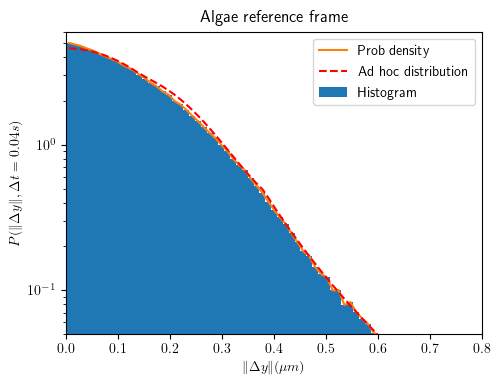
\includegraphics[width=0.4\textwidth]{archivos/pdf_ylog_e3.png}
	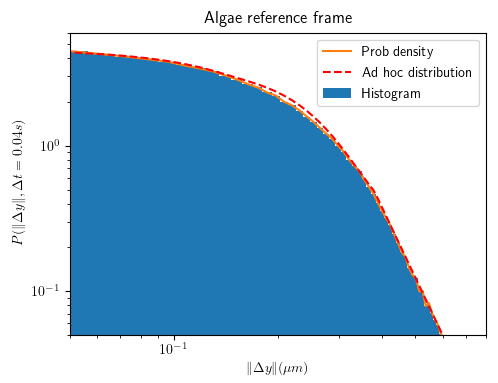
\includegraphics[width=0.4\textwidth]{archivos/pdf_loglog_e3.png}
	\caption{Fitting of the \textit{ad hoc} probability distribution function of the displacement $|\Delta y|$, (perpendicular to the algae direction vector) in the turning reference frames attached to the algae, for a fixed $\Delta t = 0.04 \; \textrm{s}$ and $\Phi = 0.674$ ($\sigma \simeq 0.15733 \; \mu \textrm{m}$, $lim_{pl}=0.13 \; \mu \textrm{m}$, $lim_g=0.38 \; \mu \textrm{m}$, $C_g \simeq 0.90863$, $C_{pl} \simeq 0.00386$, $k = 0$, $\beta = 2.84$, $\alpha = 5$)}
	\label{e3_adhoc}
\end{figure}

Regarding the results of Kurtuldu et al.~\cite{Kurtuldu2011}, we already mentioned that the scales of the distribution are affected by the studied kind of motion (pushers instead of pullers), but we also obtain a steeper descent of the Power Law tails (the exponent is $-5$ instead of $-4$). This could be logic if the energy of the kicks is lower, which seems to be the case. We will later see what happens in the case of pushers.

Another result that needs to be assessed is represented in Fig. \ref{msd_E3}. It shows the mean square tracer displacements (in the relative frame) as a function of  $\Delta t$ for different values of concentration (i.e. different circles). The mean square tracer displacement is defined as:

\begin{equation}
MSD = \frac{\displaystyle\sum_{n} \Delta x ^ 2 + \Delta y ^ 2}{n}
\end{equation}

where $n$ is the number of events. 

We are going to make the hypothesis that diffusion enhancement is isotropic (i.e. similar along $X$ and $Y$ axes). Since the motion of the algae and the background flow are ballistic along $X$ and zero in $Y$ (because of the definition of the mobile reference frame), this implies:

\begin{equation}
\Delta x = O(\Delta y) + \| \mathbf{v}_{alga} + \mathbf{v}_{bf} \| \Delta t
\end{equation}

We only want to measure diffusion, so, given the number of events is a statistically representative sample, we can write:

\begin{equation}
MSD \simeq \frac{2 \displaystyle\sum_{m} \Delta y^{2}}{n}
\label{yMSD}
\end{equation}

The MSD as defined by Eq. \ref{yMSD} is represented in Fig. \ref{MSD_e3} as a function of the elapsed time:

\begin{figure}[H]
	\centering
	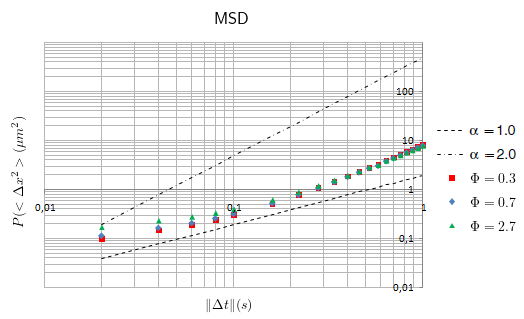
\includegraphics[width=0.6\textwidth]{archivos/MSD_e3.png}
	\caption{Mean square displacement in the turning reference frames attached to the algae as a function of $\Delta t$, for different values of $\Phi$}
	\label{MSD_e3}
\end{figure}

The behavior for $\Delta t$ under $\sim 0.1 \; \textrm{s}$ is hard to explain on a physical basis. The most plausible explanation is that, although the tracking algorithm has a theoretical precision well under the pixel ($1 \; \textrm{pixel} ~ 0.425 \; \mu \textrm{m}$), the images might be too noisy for it to work properly.

Regarding higher $\Delta t$ values, and ignoring the fact that $\Phi = 2.7\%$ is too high a concentration to be considered as belonging to the dilute limit, it is here that another problem of this methodology emerges: considering only the particles within the circles surrounding the algae may act as a filter for the long displacements. It is hard to define a cut-off length, but, since we only consider the particles that remain within a specific circle during the selected time lapse, we can say that it has to be smaller than the circle diameter. This might partially explain the convergence of the curves for different values of concentration.

As a conclusion, our numerical approach for removing the \textit{background flow} does not provide the expected results.

\section{Long-lasting films}

To summarize last section: we will set thicker films and wait for them to thin thanks to evaporation.

Just after having decided to do so, the device got damaged and we had to build a provisional one. Since we were less concerned about being precise in the initial thickness, the new device lacked of mechanisms: the threads, already in their final (stretched) position, are immersed in the solution and a film is formed between them when the device is removed vertically.

To our surprise, when the initial thickness was too high (of the order of $100 \mu \textrm m$) and, therefore, the evaporation time too long (around 1-2 hours), the algae would stop moving before we could reach the desired thickness. On the contrary, if thickness was too low, \textit{background flows} appeared again.

Several experiences were carried out to determine if the algae were dying because of a lack or excess of Oxygen or nutrients, but the results were inconclusive. 

In fact, we could not be sure if they were dying or they were only losing their flagella\footnote{In some images we appreciated detached flagella at the surface of the film. However, it is difficult to find out if algae which are not moving still have theirs.} (which can grow again in approximately one hour). The second option could have different explanations from the ones explaining death events, so it seemed appropriate to try to find out which was the case.

In order to do so, we decided to conduct a LIVE/DEAD Cell test, consisting in staining both, and which is explained in section ¿¿¿7.7???. This test did not provide the expected results for two reasons: \textit{calcein AM} seems not to be able to penetrate the algae wall, which prevents the detection of living cells; and chlorophyll is autofluorescent in the red, so it is impossible to know if we are looking at it or at \textit{EthD-1} (i.e. the dye for the dead cells, which also emits in the red spectrum).

In the end, time seemed to be more critical than thickness so, by removing the box cover in the beginning, evaporation was accelerated. Then for the last part of evaporation, the box was closed. This way, we managed to have some exploitable images without background flow and with living algae.

\section{Quiescent beads}
 
In their papers, Kurtuldu et al.~\cite{Kurtuldu2011} and Guasto et al.~\cite{Guasto} use small concentrations of surfactants to help lower the surface tension of the mixture. This facilitates the formation of the layer, whereas, theoretically, such low concentrations should not modify the general behavior of the experiment.

Nevertheless, in their article about the influence of surfactants on the drag
reduction of superhydrophobic surfaces, ¿¿¿ Peaudecerf et al.??? demonstrate that extremely low concentrations, that are present in most fluids, have huge effects on the air–liquid interface, to the point of immobilizing it. This is due to the triggering of the Marangoni effect, that is shown in the next figure:

\begin{figure}[H]
	\centering
	\includegraphics[width=0.7\textwidth]{archivos/Marangoni.png}
	\caption[Caption]{Marangoni effect in an air-water interface \textcolor{red}{¿¿¿CITE???}\protect\footnotemark caused by the presence of surfactant traces in the presence of an external flow}
	\label{Marangoni}
\end{figure}

\footnotetext{In the article, a superhydrophobic surface is represented but this does not affect the explanation.}

The presence of an external flow, which in our case could be the one generated by the breaststroke motion of the algae, generates gradients of surfactants. Since surfactants diminish the surface tension, this generates forces that oppose to this flow on the surface (Marangoni forces), altering its motion, which would, otherwise, follow that of the bulk.

This phenomena can be understood as a \textit{rigidization} of the surface, because it gives rise to parabolic velocity profiles within our layer.

All of the above could explain one of the problems we have come across during this research: some of the tracers would simply not move. Not even in a brownian way. In Fig. \ref{quiescent_beads}, we can observe some streamlines that reveal the \textit{quiescent beads}.  

\begin{figure}[H]
	\centering
	\includegraphics[width=0.4\textwidth]{archivos/190726_H2O_0_18p5um_0001.png}
	\includegraphics[width=0.4\textwidth]{archivos/190726_H2O_0_18p5um_MIN200.png}
	\caption{Quiescent beads (yellow circles) are shown in one frame (left) and its streamlines (right) for $4 \; \textrm{seconds}$ (no surfactants were added in this experiment)}
	\label{quiescent_beads}
\end{figure}

This happened in experiments where we had added no surfactant to the solution. We infer that the algal biological activity may generate some of it and, that even if it does not, it would be impossible to get completely rid of these substances.

We also know that even if the effect is not that extreme, diffusion at the interfaces is lower than in the bulk (see, for instance,~\cite{peng2009}). Moreover, our tracers will slowly sediment to the bottom interface exacerbating this trend. There does not seem to be a solution to avoid particle accumulation at the interfaces, but sedimentation can be avoided thanks to density matching. For this purpose, either  $\sim 1 \; \textrm{g/cc}$ dense spheres can be acquired or the medium can be mixed with glycerol or heavy water. Glycerol increases the viscosity of the solution, which could alter our results, so we have dismissed this option. Heavy water is probably toxic for \textit{Chlamydomonas}, but they may not be affected in the time scale of our experiment so we might consider using it in the future. Otherwise, we will try to take this factors into account when processing the data if they disturb the statistics.

\section{Last results}

After the long process described up to now in this section, we managed to get two sets of images that did not show any of the mentioned issues.

The first of them corresponds to a $\sim 20 \; \mu \textrm{m}$ thick film, and a concentration $\Phi \simeq 2.42\%$.

For long enough times, we can see that the $|\Delta x|$ distribution is almost perfectly Gaussian:

\begin{figure}[H]
	\centering
	\includegraphics[width=0.4\textwidth]{archivos/GaussXpdf_ylog_Dt076_ANH_Chlamy_beads_Thickness18pt_60x.png}
	\includegraphics[width=0.4\textwidth]{archivos/GaussXpdf_loglog_Dt076_ANH_Chlamy_beads_Thickness18pt_60x.png}
	\caption{Fitting of a Gaussian to the probability distribution function of the displacement $|\Delta x|$, in the absolute reference frame, for a fixed $\Delta t = 0.76 \; \textrm{s}$ and $\Phi = 2.42\%$ ($\sigma \simeq 4.578865732063 \; \mu \textrm{m}$)}
	\label{ANH_Gauss_X}
\end{figure}

For lower times, the tails are not Gaussian anymore (see Fig. \ref{ANH_Tails}).

%\begin{figure}[H]
%	\centering
%	\includegraphics[width=0.4\textwidth]{archivos/GaussYpdf_ylog_Dt076_ANH_Chlamy_beads_Thickness18pt_60x.png}
%	\includegraphics[width=0.4\textwidth]{archivos/GaussYpdf_loglog_Dt076_ANH_Chlamy_beads_Thickness18pt_60x.png}
%	\caption{Fitting of a Gaussian to the probability distribution function of the displacement $|\Delta y|$, in the absolute reference frame, for $\Phi = 2.42\%$ ($\sigma \simeq 5.149580504573869 \mu m$)}
%	\label{ANH_Gauss_Y}
%\end{figure}

\begin{figure}[H]
	\centering
	\includegraphics[width=0.6\textwidth]{archivos/TailsANH.png}
	\caption{Normalized probability distribution function of the displacement $|\Delta x|$, in the absolute reference frame, for $\Phi = 2.42\%$. The value of the exponent is $a=5.8$ for the Power Law and $\sigma \simeq 5.149580504573869 \mu m$ for the Gaussian distribution.}
	\label{ANH_Tails}
\end{figure}

As suggested by Kurtuldu et Al.~\cite{Kurtuldu2011}, tails seem to have a potential character: their slope is constant in logarithmic axes. As it can be seen on Fig. \ref{ANH_Tails}), this slope changes with  $\Delta t$, approaching the Gaussian distribution for higher values of this variable.

As we have already mentioned, the noise on the images makes it very hard to obtain valid data for $\Delta t$ under a certain threshold. This threshold's seems to be around $0.06 \; \textrm{s}$ (see Fig. \ref{MSD_ANH}). Consequently, we have only been able to measure the exponent's value for $\Delta t = 0.08 \; \textrm{s}$, which is approximately $-5.8$. This value, although far from the $-4$ obtained by Kurtuldu et Al.~\cite{Kurtuldu2011}, suggests that for lower elapsed times we can, in fact, expect something of the order of $-4$.

We can now have a look at the MSD:

\begin{figure}[H]
	\centering
	\includegraphics[width=0.6\textwidth]{archivos/MSD_ANH.png}
	\caption{Mean square displacement in the absolute reference frame as a function of $\Delta t$, for different values of $\Phi$}
	\label{MSD_ANH}
\end{figure}

The above described experiment corresponds to the blue dots, whereas the red ones have been obtained from a second exploitable set of images\footnote{Conclusions from both sets are very similar, so, for the sake of brevity, we will not further explore this data set here.}. 

We can see that the data for $\Delta t$ under $0.06 \; \textrm{s}$ draw a curve whose growth is slower than the one expected for Brownian motion. Since we can see no physical reason for this to happen, we put this error down to a precision matter, probably due to noise in the images.

Data over that threshold show a superdiffusive trend, with slopes $\sim 1.5 - 1.6$, that relax towards a normal diffusive scaling at higher values of $\Delta t$ when the distributions become Gaussian (this is more easily appreciated on the blue curve).

\textcolor{red}{¿¿¿ LOOK FOR DIFFUSION COEFS IF I HAVE THE TIME ???}

	\chapter{Conclusions}
\label{conclusions}

In this section we will go through the posed objectives and asses the level of observance for each of them.

\section{Acquaintance with bibliography on the matter}

The cited papers are very few compared to the many we have dealt with, and much fewer compared to the existing bibliography on the topic. Consequently, full compliance on this matter is impossible to achieve. Yet, we have found a lot of the answers to our questions among the pages of the cited documents, which has saved us a lot of time.

\section{Algae culture and handling}

In spite of some contamination related issues, we have managed to maintain a constant supply of \textit{Chlamydomonas reinhardtii}, allowing the realization of experiments on a regular basis. 

\section{Device design and construction}

The initial development of our was a quick process: in less than two weeks we were already performing the first experiences. However, upgrades to this initial idea have been implemented all throughout the project.

Unfortunately, at a certain point, the device was damaged and a temporary solution had to be devised. This improvised solution turned out to be rather effective and even inspired some of the protocols that we would finally apply to deal with the problem of \textit{background flows}.

\section{Image acquisition}

Although we are indeed using fluorescent beads, the intensity of the autofluorescence of \textit{Chlamydomonas reinhardtii}, provided by its chlorophyll, is not enough to consider fluorescence microscopy as an option.

By means of light microscopy, in the end we seem to have managed to obtain at least two sets of images where the motion of algae and tracers is not-biased, either by background flows or other factors. Yet, probably because of the noise, we have not been able to properly analyze very small displacements with the selected tracking algorithm. This means that further image processing is to be done and tested.

The selected technique is particle tracking velocimetry (PTV), but the resulting images should also be valid for other velocity measuring techniques such as particle image velocimetry (PIV). This technique (PIV) should be explored in future works to find out its advantages and disadvantages, compared to PTV, when applied to the analysis of our images.

\section{Particle tracking}


\textcolor{red}{We intend to develop a Python code that will allow an automation of the image processing needed to improve the performance of the selected tracking algorithm. Such algorithm, originally implemented by John Crocker and Eric Weeks~\cite{Crocker} in Interactive Data Language (IDL) has been reimplemented in a Python
open library under the name Trackpy. Our code will call on that library and save the trajectories and other derived data in text files to be analyzed later.}

\section{Data analysis}

The information revealed up to now by our data seems to be in agreement with previous literature on the topic (mainly~\cite{Kurtuldu2011}). Nonetheless, further analysis of the data is still required. 

Once this analysis will be completed, a similar one must be conducted on data obtained from thicker layers, since the numerical model is currently unable to deal with 2D systems\footnote{For systems under a certain, the fictitious forces playing the role of boundary conditions cane explode numerically when two swimmers meet.}.

\section{Side phenomena explanation}

Three side phenomena have been of our main interest, since they prevented us from acquiring exploitable images: background flows, quiescent beads and premature algal death/loss of flagella.

The first of this phenomena has been explained in this document and successfully mitigated. The second one, although explicable, seems to be unavoidable in our experiments, so we need to make sure it does not affect our results. The third one has not yet been understood, but can be avoided in a rather simple way.

\section{Conclusions and open-ended questions}

\textcolor{red}{¿¿¿ Pushers ???}

\textcolor{red}{This project is headed to draw a set of qualitative and quantitative conclusions concerning the enhanced mixing generated by \textit{Chlamydomonas reinhardtii} in a 2D environment. It is also our intention to transfer the acquired knowledge to 3D configurations in order to find out the differences induced by dimensionality. Last, but not least, the emerging and unanswered questions will be put on paper to inspire future works.}
	
	%\includepdf[pages={57-97}]{archivos/plantilla-tfg-fium.pdf}

	
	%%%%
	% CONTENIDO. BIBLIOGRAFÍA.
	%%%%
	\nocite{*} %incluye TODOS los documentos de la base de datos bibliográfica sean o no citados en el texto
	\bibliographystyle{unsrtnat}
	\bibliography{bibliography/bibliography} % Archivo que contiene la bibliografía
	
	
	%%%%
	% CONTENIDO. LISTA DE ACRÓNIMOS. Comenta las líneas si no lo deseas incluir.
	%%%%
	% Incluye el listado de acrónimos utilizados en el trabajo. 
	\printglossary[style=modsuper,type=\acronymtype,title={List of Acronyms}]
	% Añade el resto de acrónimos si así se desea. Si no elimina el comando siguiente
	\glsaddallunused
	
	%%%%
	% CONTENIDO. Anexos - Añade o elimina según tus necesidades
	%%%%
	\appendix % Inicio de los apéndices
	\chapter{Anexo I}

\section{Tablas}

\begin{table}[H]
	\begin{tabular}{llll}
		\cline{1-2}
		\multicolumn{1}{|l|}{FRAMES} & \multicolumn{1}{c|}{2699} & & \\ \cline{1-2}
		\multicolumn{1}{|l|}{PARTICLES} & \multicolumn{1}{c|}{870} & & \\ \cline{1-2}
		&  &  &  \\ \cline{1-1}
		\multicolumn{1}{|l|}{EVENTS} &  &  &  \\ \hline
		\multicolumn{1}{|l|}{$\Delta t \; \textrm{(s)}$ \textbackslash $\Phi (\%)$} & \multicolumn{1}{c|}{$0.3\%$} & \multicolumn{1}{c|}{$0.7\%$} & \multicolumn{1}{c|}{$2.7\%$} \\ \hline
		\multicolumn{1}{|l|}{0,02} & \multicolumn{1}{c|}{1301925} & \multicolumn{1}{c|}{621481} & \multicolumn{1}{c|}{177681}\\ \hline
		\multicolumn{1}{|l|}{0,04} & \multicolumn{1}{c|}{1297358} & \multicolumn{1}{c|}{619311} & \multicolumn{1}{c|}{176979}\\ \hline
		\multicolumn{1}{|l|}{0,06} & \multicolumn{1}{c|}{1292804} & \multicolumn{1}{c|}{617143} & \multicolumn{1}{c|}{176283}\\ \hline
		\multicolumn{1}{|l|}{0,08} & \multicolumn{1}{c|}{1288262} & \multicolumn{1}{c|}{614980} & \multicolumn{1}{c|}{175590}\\ \hline
		\multicolumn{1}{|l|}{0,1} & \multicolumn{1}{c|}{1283731}  & \multicolumn{1}{c|}{612817} & \multicolumn{1}{c|}{174894}\\ \hline
		\multicolumn{1}{|l|}{0,16} & \multicolumn{1}{c|}{1270226} & \multicolumn{1}{c|}{606354} & \multicolumn{1}{c|}{172818}\\ \hline
		\multicolumn{1}{|l|}{0,22} & \multicolumn{1}{c|}{1256800} & \multicolumn{1}{c|}{599922} & \multicolumn{1}{c|}{170753}\\ \hline
		\multicolumn{1}{|l|}{0,28} & \multicolumn{1}{c|}{1243462} & \multicolumn{1}{c|}{593558} & \multicolumn{1}{c|}{168700}\\ \hline
		\multicolumn{1}{|l|}{0,34} & \multicolumn{1}{c|}{1230237} & \multicolumn{1}{c|}{587236} & \multicolumn{1}{c|}{166655}\\ \hline
		\multicolumn{1}{|l|}{0,4} & \multicolumn{1}{c|}{1217170}  & \multicolumn{1}{c|}{580987} & \multicolumn{1}{c|}{164631}\\ \hline
		\multicolumn{1}{|l|}{0,46} & \multicolumn{1}{c|}{1204352} & \multicolumn{1}{c|}{574856} & \multicolumn{1}{c|}{162647}\\ \hline
		\multicolumn{1}{|l|}{0,52} & \multicolumn{1}{c|}{1191601} & \multicolumn{1}{c|}{568753} & \multicolumn{1}{c|}{160659}\\ \hline
		\multicolumn{1}{|l|}{0,58} & \multicolumn{1}{c|}{1183141} & \multicolumn{1}{c|}{564710} & \multicolumn{1}{c|}{159337}\\ \hline
		\multicolumn{1}{|l|}{0,64} & \multicolumn{1}{c|}{1166410}   & \multicolumn{1}{c|}{556721} & \multicolumn{1}{c|}{156730}\\ \hline
		\multicolumn{1}{|l|}{0,7} & \multicolumn{1}{c|}{1154002}  & \multicolumn{1}{c|}{550804} & \multicolumn{1}{c|}{154799}\\ \hline
		\multicolumn{1}{|l|}{0,76} & \multicolumn{1}{c|}{1141772} & \multicolumn{1}{c|}{544968} & \multicolumn{1}{c|}{152908}\\ \hline
		\multicolumn{1}{|l|}{0,82} & \multicolumn{1}{c|}{1129692} & \multicolumn{1}{c|}{539189} & \multicolumn{1}{c|}{151043}\\ \hline
		\multicolumn{1}{|l|}{0,88} & \multicolumn{1}{c|}{1117701} & \multicolumn{1}{c|}{533437} & \multicolumn{1}{c|}{149179}\\ \hline
		\multicolumn{1}{|l|}{0,94} & \multicolumn{1}{c|}{1105801} & \multicolumn{1}{c|}{527726} & \multicolumn{1}{c|}{147335}\\ \hline
		\multicolumn{1}{|l|}{1} & \multicolumn{1}{c|}{1094020} & \multicolumn{1}{c|}{522066} & \multicolumn{1}{c|}{145508}\\ \hline
	\end{tabular}
	\caption{¿¿¿CAPTION E3???}
	\label{table_e3}
\end{table}

\begin{table}[H]
	\begin{tabular}{ll}
		\hline
		\multicolumn{1}{|l|}{FRAMES} & \multicolumn{1}{c|}{2726} \\ \hline
		\multicolumn{1}{|l|}{PARTICLES} & \multicolumn{1}{c|}{2352} \\ \hline
		&  \\ \cline{1-1}
		\multicolumn{1}{|l|}{EVENTS} &  \\ \hline
		\multicolumn{1}{|l|}{$\Delta t \; \textrm{(s)}$ \textbackslash $\Phi (\%)$} & \multicolumn{1}{c|}{$2.42\%$} \\ \hline
		\multicolumn{1}{|l|}{0,02} & \multicolumn{1}{c|}{301696} \\ \hline
		\multicolumn{1}{|l|}{0,04} & \multicolumn{1}{c|}{299344} \\ \hline
		\multicolumn{1}{|l|}{0,06} & \multicolumn{1}{c|}{296992} \\ \hline
		\multicolumn{1}{|l|}{0,08} & \multicolumn{1}{c|}{294640} \\ \hline
		\multicolumn{1}{|l|}{0,1}  & \multicolumn{1}{c|}{292288} \\ \hline
		\multicolumn{1}{|l|}{0,16} & \multicolumn{1}{c|}{285232} \\ \hline
		\multicolumn{1}{|l|}{0,22} & \multicolumn{1}{c|}{278176} \\ \hline
		\multicolumn{1}{|l|}{0,28} & \multicolumn{1}{c|}{271120} \\ \hline
		\multicolumn{1}{|l|}{0,34} & \multicolumn{1}{c|}{264064} \\ \hline
		\multicolumn{1}{|l|}{0,4}  & \multicolumn{1}{c|}{257008} \\ \hline
		\multicolumn{1}{|l|}{0,46} & \multicolumn{1}{c|}{249952} \\ \hline
		\multicolumn{1}{|l|}{0,52} & \multicolumn{1}{c|}{242896} \\ \hline
		\multicolumn{1}{|l|}{0,58} & \multicolumn{1}{c|}{238192} \\ \hline
		\multicolumn{1}{|l|}{0,64} & \multicolumn{1}{c|}{228784} \\ \hline
		\multicolumn{1}{|l|}{0,7}  & \multicolumn{1}{c|}{221728} \\ \hline
		\multicolumn{1}{|l|}{0,76} & \multicolumn{1}{c|}{214672} \\ \hline
		\multicolumn{1}{|l|}{0,82} & \multicolumn{1}{c|}{207616} \\ \hline
		\multicolumn{1}{|l|}{0,88} & \multicolumn{1}{c|}{200560} \\ \hline
		\multicolumn{1}{|l|}{0,94} & \multicolumn{1}{c|}{193504} \\ \hline
		\multicolumn{1}{|l|}{1}    & \multicolumn{1}{c|}{186448} \\ \hline
	\end{tabular}
	\caption{¿¿¿CAPTION ANH???}
	\label{table_ANH}
\end{table}

\begin{table}[H]
	\begin{tabular}{ll}
		\hline
		\multicolumn{1}{|l|}{FRAMES} & \multicolumn{1}{c|}{2726} \\ \hline
		\multicolumn{1}{|l|}{PARTICLES} & \multicolumn{1}{c|}{2269} \\ \hline
		&  \\ \cline{1-1}
		\multicolumn{1}{|l|}{EVENTS} &  \\ \hline
		\multicolumn{1}{|l|}{$\Delta t \; \textrm{(s)}$ \textbackslash $\Phi (\%)$} & \multicolumn{1}{c|}{$2.42\%$} \\ \hline
		\multicolumn{1}{|l|}{0,04} & \multicolumn{1}{c|}{417045}\\ \hline
		\multicolumn{1}{|l|}{0,06} & \multicolumn{1}{c|}{414776}\\ \hline
		\multicolumn{1}{|l|}{0,08} & \multicolumn{1}{c|}{412507}\\ \hline
		\multicolumn{1}{|l|}{0,1}  & \multicolumn{1}{c|}{410238}\\ \hline
		\multicolumn{1}{|l|}{0,02} & \multicolumn{1}{c|}{407969}\\ \hline
		\multicolumn{1}{|l|}{0,16} & \multicolumn{1}{c|}{401162}\\ \hline
		\multicolumn{1}{|l|}{0,22} & \multicolumn{1}{c|}{394355}\\ \hline
		\multicolumn{1}{|l|}{0,28} & \multicolumn{1}{c|}{387548}\\ \hline
		\multicolumn{1}{|l|}{0,34} & \multicolumn{1}{c|}{380741}\\ \hline
		\multicolumn{1}{|l|}{0,4}  & \multicolumn{1}{c|}{373934}\\ \hline
		\multicolumn{1}{|l|}{0,46} & \multicolumn{1}{c|}{367127}\\ \hline
		\multicolumn{1}{|l|}{0,52} & \multicolumn{1}{c|}{360320}\\ \hline
		\multicolumn{1}{|l|}{0,58} & \multicolumn{1}{c|}{355782}\\ \hline
		\multicolumn{1}{|l|}{0,64} & \multicolumn{1}{c|}{346706}\\ \hline
		\multicolumn{1}{|l|}{0,7}  & \multicolumn{1}{c|}{339899}\\ \hline
		\multicolumn{1}{|l|}{0,76} & \multicolumn{1}{c|}{333092}\\ \hline
		\multicolumn{1}{|l|}{0,82} & \multicolumn{1}{c|}{326285}\\ \hline
		\multicolumn{1}{|l|}{0,88} & \multicolumn{1}{c|}{319478}\\ \hline
		\multicolumn{1}{|l|}{0,94} & \multicolumn{1}{c|}{312671}\\ \hline
		\multicolumn{1}{|l|}{1}    & \multicolumn{1}{c|}{305864}\\ \hline
	\end{tabular}
	\caption{¿¿¿CAPTION ANHlt???}
	\label{table_ANHlt}
\end{table}


	%% Ejemplo de páginas en horizontal y vertical

\chapter{Páginas horizontales}
Aquí se muestra cómo incluir páginas en horizontal.

Esta página está en vertical\\
\clearpage % Nueva página

\begin{landscape} % Inicia modo horizontal
	

Esta página está en horizontal\\
\clearpage % Nueva página

Esta página también está en horizontal\\

\end{landscape} % Finaliza modo horizontal
\clearpage % Nueva página


Esta página está de nuevo en vertical\\




	%% Ejemplo de inclusión de páginas de un PDF

\chapter{Importar PDF}

A continuación se muestra una página importada de un PDF externo. Observar los comentarios en el código de este anexo para más información. También puedes leer el manual con todas las opciones en \url{http://osl.ugr.es/CTAN/macros/latex/contrib/pdfpages/pdfpages.pdf}.

%\includepdf[pages={1}]{archivos/ES_a_DF7_Agg_Alicante.pdf}

% Para incluir una página:
% [pages={0}] % Donde '0' es el número de la pagina del PDF que se quiere incluir

% Para incluir varias páginas consecutivas
% [pages={1-4}] % Con estos valores importa de la página 1 a la 4.

% Para incluir varias páginas salteadas
% [pages={1,4,7,10}] % Incluye las páginas 1,4,7 y 10

% Para incluir todo el documento PDF
% [pages=-]

% Si ademas de pages=... se incluye landscape, se importa en horizontal
% [pages{1},landscape]

----------------------------------

Why: basic research, confirming numerical results, any possible applications
State of the art

Active suspensions (examples)
Chlamydomonas reinhardtii description
Culture \& species

Fluid mechanics
Microfluidics (Reynolds) - (Distributions --> Weighed sum??)
Fluid field around a cell 
Brownian motion and advection (Peclet number)

Materials and methods
Devices
Microscope, red filter (other possibilities: fluorescence)
High-speed videocamera
Particle-tracking algorithm
Concentration: Hemocytometer, circles
Code

Problems
Equations soap film --> Thickness importance

	
\end{document}